\chapter{The Kinetic Guarantee: Arms Asymmetry, the Second Amendment, and the Disarmament Timeline}
\label{ch:kinetic}

\begin{tcolorbox}[colback=black!5, colframe=black!70, fonttitle=\bfseries\ttfamily, title=RUNTIME LOG: TRACING THE DISARMAMENT VARIABLE ACROSS THE FULL TIMELINE]
\ttfamily\small
\textbf{System Origin}: Portuguese firearms superiority (1440s) --- technological asymmetry in lethal capacity enables mass extraction.\\
\textbf{Feedback Loop Detected}: Arms-for-slaves trade creates exponential demand. Firearms $\rightarrow$ military advantage $\rightarrow$ captives $\rightarrow$ currency for more firearms.\\
\textbf{Interference State} ($\Phi_{\text{load}}$, proximity to $\tau$): MODERATE-HIGH --- disarmament operates as kinetic adjunct to identity-fragmentation controls. Estimated $\Phi_{\text{load}} \in [0.60, 0.85]$, $\rho_{\tau} \in [0.70, 0.95]$.\\
\textbf{Constitutional Encoding}: Second Amendment (1791) --- kinetic guarantee installed as dead man's switch. Racial and gendered exclusions baked into source code.\\
\textbf{Disarmament Protocol}: Sullivan Law (1911) $\rightarrow$ NFA (1934) $\rightarrow$ Mulford Act (1967) $\rightarrow$ GCA (1968) $\rightarrow$ Hughes Amendment (1986) $\rightarrow$ Brady/AWB (1993--94; causative context at $\S$\ref{sec:ruby_ridge_waco}) $\rightarrow$ Post-Bruen state responses (2022--present).\\
\textbf{Agenda Routing}: Under elevated $\Phi_{\text{load}}$, policy sequence moves from targeted controls on $O_{\text{racialized}}$ to generalized controls on $I_{\text{buffer}}$ through cumulative jurisprudential precedent.\\
\textbf{PATTERN}: Every federal gun control law correlates with either (a) $O_{\text{racialized}}$ approaching kinetic parity or (b) $P_{\text{uppet}}$ members being kinetically corrected. The disarmament variable is a \textbf{pillar} of the extraction kernel; the policy debate is its surface framing.
\end{tcolorbox}

\paragraph{Primary statutory text (machinegun transfer bar, Hughes).}
The post-1986 machinegun provisions appear at \usclink{apx:usc:18:922o}{18 U.S.C.~\S922(o)}:
\uscinline{usc_18_922o}

\medskip

The preceding chapters have traced the Predatory Min-Max Function through its legal, economic, spatial, and psychological variables. The framework has not yet isolated the variable that \textit{precedes all others}---the one without which the entire five-century extraction apparatus could not have been initialized. That variable is \textbf{asymmetric lethal capacity}: the technological gap in the ability to inflict organized violence.

Every extraction system documented in this book---chattel slavery, convict leasing, redlining, the carceral state---depends on the same precondition: the extracting class must possess a monopoly, or near-monopoly, on the capacity to kill. If the extracted population can fight back with equivalent force, the extraction equation collapses. The entire history of gun control in America---from the colonial era to the post-Bruen state responses of 2022--present---is the history of the Elite managing this single variable.

This chapter traces the disarmament variable from its origin to the present day, demonstrating that ``gun control'' is a continuous, five-century operation to maintain the lethal asymmetry without which the Predatory Min-Max Function cannot execute. The public-safety framing is a modern policy debate; the underlying operation is five centuries old.

The kinetic variable matters because a mind virus persists even when hosts are shown the contradiction. Hosts can still defend the prior if the enforcement environment makes dissent physically impossible or individually irrational. Disarmament therefore functions as the hard-power companion to cognitive infection: it ensures that even when the host wetware begins to reject the malicious prior, the extraction kernel still owns the means of compulsion.

\section{The Firearms Asymmetry: How Guns Created the African Diaspora}

The African diaspora exists outside Africa \textit{because of guns}.

This claim requires substantiation, but the historical record is unambiguous. When Portuguese traders first made contact with West African kingdoms in the mid-15th century, the technological gap in military capacity was decisive. European firearms---crude by later standards but devastating against populations that had not developed gunpowder weapons---provided the asymmetric lethal advantage that enabled mass kidnapping and, eventually, the transatlantic slave trade \cite{thornton}.

The extraction operated in two phases.

\subsection{Phase 1: Direct Kidnapping Through Firearms Superiority}

The earliest Portuguese slave raids on the West African coast relied on a simple calculus: a small number of armed men with firearms could overpower a larger number of defenders wielding edged and projectile weapons that could not match the range, lethality, or psychological impact of gunfire. This technological asymmetry was the \textit{enabling condition} for the transatlantic slave trade. Racial superiority, cultural destiny, and divine mandate supplied the ideological defense; the military gap supplied the operational precondition. Without the gun, the extraction pipeline could not have been initialized.

The framework must identify \textit{why} the asymmetry existed in the first place, because the system's ideological defense (Component~3) has historically attributed European military superiority to racial or civilizational destiny. The actual cause was structural and contingent: \textbf{centuries of relentless European internecine warfare}. The Hundred Years' War (1337--1453), the Italian Wars, the Reconquista, the Hussite Wars, the Wars of the Roses---Europe spent the 14th and 15th centuries in near-continuous state-on-state armed conflict. This perpetual warfare created an arms race among European powers that drove the rapid iteration and refinement of gunpowder weapons, siege technology, naval armaments, and military logistics. By the time Portuguese ships reached the West African coast in the 1440s, European firearms technology had been forged through a century of competitive military selection pressure that West African societies---whose military traditions were adapted to their own geopolitical contexts, including highly effective cavalry, iron-working, fortification, and organized infantry---had not been subjected to.

The technological gap was confined to military technology. West African kingdoms possessed sophisticated metallurgy, agricultural engineering, urban planning, and trade networks that rivaled or exceeded their European contemporaries. The Malian Empire's Mansa Musa had destabilized the gold markets of Cairo and Medina two centuries before the Portuguese arrived. The gap was narrowly military-technological, produced by the specific selection pressure of European infighting, and it was \textit{temporary}---within decades, West African kingdoms were acquiring, adapting, and in some cases manufacturing firearms. The window of asymmetry was sufficient to initialize the extraction pipeline, and once the arms-for-slaves feedback loop was established, the system no longer required direct European superiority to sustain itself.

The framework's notation captures this precisely. Let $L_E$ denote the lethal capacity of the Elite and $L_O$ the lethal capacity of the target population. The extraction precondition is:
\begin{equation}\label{eq:11.1-extraction-precondition}
L_E \gg L_O \implies \text{Extraction feasible}
\end{equation}

When this inequality holds, $E$ can impose the full oppressive architecture: asymmetric power (Component~1), resource extraction (Component~2), ideological justification (Component~3), and resistance suppression (Component~4). When $L_O \to L_E$---when the target population approaches lethal parity---the extraction equation destabilizes. The entire history of gun control is the history of maintaining the inequality $L_E \gg L_O$ after the initial technological gap began to close.

\subsection{The State Cartel: Monopoly on Violence as Semantic Legitimation}

The state monopoly on violence is usually described as legitimacy: the state claims the exclusive right to authorize coercive force within its territory \cite{weber_politics_vocation}. The framework reads the same fact as a semantic exploit. The institutional node that performs an action determines its name, while the material structure---taking property, confining bodies, threatening force, or killing at scale---remains constant.

\begin{equation}\label{eq:11.1a-state-semantic-legitimation}
\operatorname{Name}(a)=
\begin{cases}
\text{taxation, justice, security} & a \in A_{\text{state}} \text{ and } S_{\text{legit}}=1,\\
\text{extortion, kidnapping, assault} & a \in A_{\text{civilian}} \text{ and } S_{\text{legit}}=0.
\end{cases}
\end{equation}

The semantic label changes; the kinetic substrate does not. A private actor who seizes wages under threat commits extortion, while a state-enabled wage-theft regime can drain billions through procedural delay, weak enforcement, and civil penalties too small to deter extraction. A private actor who poisons a neighborhood commits assault or murder, while regulatory capture can expose entire communities to lead, particulates, and industrial toxins through permits, variances, and non-enforcement. A private actor who cages a person commits kidnapping, while the carceral state converts the same deprivation of liberty into ``justice'' and then routes labor through the 13th Amendment exception clause.

This distinction identifies the scale problem; uncoordinated civilian violence remains real. Civilian violence is local, episodic, and usually legible as crime. State violence is industrial, recursive, and pre-labeled as order before the victim can contest it. The monopoly on violence functions as a compilation layer that translates coercion into legality. Kinetic parity matters because it is the only variable that forces the state-cartel node to abandon inventory pricing and treat the governed as agents.

\subsection{Phase 2: The Arms-for-Slaves Feedback Loop}

The second phase was more insidious---and more profitable. As the slave trade matured, the Portuguese and subsequently the Dutch, British, and French discovered that they could \textit{weaponize the firearms asymmetry itself} as a currency system. European traders sold firearms to coastal African kingdoms, but the only currency they accepted in return was enslaved human beings \cite{inikori}.

This created an exponential feedback loop:

\begin{enumerate}
    \item European traders introduce firearms to Kingdom A.
    \item Kingdom A now possesses a decisive military advantage over neighboring Kingdom B.
    \item Kingdom B faces a choice: acquire firearms or be conquered and enslaved.
    \item The only way to acquire firearms is to provide enslaved people to the European traders.
    \item Kingdom B begins raiding Kingdom C to acquire captives to trade for firearms.
    \item The cycle propagates inland, creating an expanding wave of militarized slaving that reaches hundreds of miles from the coast.
\end{enumerate}

The mathematics are self-reinforcing. Once a single node in the system acquires firearms, every adjacent node must acquire them for defensive purposes. The only available currency is human bodies. The European Elite controlled the supply of firearms and the demand for slaves---they were both the arms dealer and the slave buyer, sitting at the apex of a system that forced African kingdoms into a coercive arms race whose fuel was their own population \cite{whatley2018}.

By the late 18th century, European traders were importing an estimated 283,000 to 394,000 firearms per year into West Africa, and the correlation between firearms imports and slave exports was direct and measurable \cite{inikori}. The feedback loop had achieved industrial scale.

\subsection{Dismantling the ``Africans Sold Themselves'' Counter-Argument}

The framework must address this counter-argument directly, because it is a pristine instantiation of $P_{\text{gaslight}}$ operating at civilizational scale.

The claim that ``Africans sold themselves into slavery'' requires the listener to perform the following cognitive operations:

\begin{enumerate}
    \item \textbf{Erase the coercive structure.} The arms-for-slaves dynamic operated under coercion. Once European firearms entered the system, participation was not optional. A kingdom that refused to trade slaves for guns would be conquered by a kingdom that did. The ``choice'' to participate was the same ``choice'' a person makes when handing over their wallet at gunpoint.

    \item \textbf{Equate fundamentally different systems.} Pre-existing forms of servitude in West African societies---war captives, debt bondage, household labor---differed structurally from chattel slavery in the Americas \cite{lovejoy2012}. They were temporary, kinship-based, or debt-based statuses; hereditary bondage, racialization, and the legal fiction of moveable property were absent. The tribes who traded captives to European slavers had no knowledge of---and no basis to anticipate---the industrial death machine of the Middle Passage and the plantation system \cite{smallwood}. Equating African domestic servitude with New World chattel slavery is like equating a bar fight with the atomic bomb because both involve violence.

    \item \textbf{Assign co-architect status to coerced participants.} The European Elite created the demand for slaves, supplied the firearms that coerced participation, built the ships, designed the plantation system, wrote the slave codes, and captured the profits. African kingdoms were \textit{nodes} in a system engineered by $E$, not co-architects of it. Blaming the coerced participants for the system that coerced them is the same logical operation as blaming the modern Out-group for the compounding effects of policies they had no hand in designing---which is precisely what $P_{\text{gaslight}}$ does domestically.
\end{enumerate}

The ``Africans sold themselves'' argument is $P_{\text{gaslight}}^{\text{kernel denial}}$ applied retroactively to the origin point of the entire extraction system---an attempt to distribute the moral burden of the slave trade across its victims in order to dilute the causal responsibility of the Elite who engineered it.

\section{The Constitutional Encoding: The Second Amendment as Kinetic Guarantee (1791)}

Chapter~\ref{ch:contradiction}'s analysis of the Framers' twenty-one confessions established that the Second Amendment was designed as a dead man's switch---a permanent kinetic guarantee ensuring that the governed retain the physical capacity to terminate the constitutional contract by force. The Framers understood, because they had just fought a revolution triggered by a disarmament attempt, that every other right in the Bill of Rights depends on the population's ability to enforce those rights through lethal capacity.

The constitutional source code contained two critical bugs from inception.

\textbf{Bug 1: The Racial Exclusion.} The Second Amendment protects ``the right of the people''---but as the Dred Scott decision would later make explicit, Black Americans were excluded from ``the people.'' The kinetic guarantee was designed to protect the Buffer Class and the white population generally; the racialized Out-group was excluded by design. This functions as a feature of the extraction kernel. The system requires $L_E \gg L_O$; granting the Out-group lethal parity would collapse the extraction equation.

\textbf{Bug 2: The Gendered Exclusion.} As documented in the preceding chapter's analysis of the Framers' language, every foundational statement of the kinetic guarantee uses gendered terms---``every man,'' ``all men capable of bearing arms.'' This exclusion operates through the identical extraction logic: denying lethal autonomy to half the population along a second partition axis ($O_{\text{gendered}}$), further fragmenting the kinetic capacity of the governed.

These bugs were load-bearing features of the extraction architecture. The Framers encoded a kinetic guarantee that protected \textit{some} of the governed against \textit{some} tyranny---specifically, the tyranny of a centralized federal government against white male property owners. The system's subsequent history is the history of selectively expanding and contracting who qualifies for the guarantee, always in service of the Predatory Min-Max Function.

\subsection{The Heller Confirmation and Its Internal Contradiction}

Two centuries after the founding, the Supreme Court was forced to settle a question the Framers would have found absurd: does the Second Amendment protect an individual right, or only a collective right tied to militia service? In \textit{District of Columbia v.\ Heller} (2008), Justice Scalia, writing for a 5--4 majority, confirmed what the twenty-one Framer statements in Chapter~\ref{ch:contradiction} make obvious: the Second Amendment protects an individual right to possess and carry weapons, unconnected with service in a militia, for traditionally lawful purposes such as self-defense \cite{heller}.

The opinion's textual analysis maps onto the framework with precision. Scalia defined the militia as ``all males physically capable of acting in concert for the common defense''---confirming Richard Henry Lee's and Madison's definitions quoted in Chapter~\ref{ch:contradiction}. He ruled that ``well-regulated'' means properly disciplined and trained---a meaning independent of government control---exactly as the Framers' own language specifies. And he identified the historical threat the amendment was designed to prevent:

\begin{quote}
``[T]he way tyrants had eliminated a militia consisting of all the able-bodied men was not by banning the militia but simply by taking away the people's arms, enabling a select militia or standing army to suppress political opponents.'' \cite{heller}
\end{quote}

Scalia wrote the thesis of this chapter in a single sentence. The disarmament timeline---from the NFA through the post-Bruen state responses---is the modern execution of exactly the tyrannical strategy the Framers encoded the Second Amendment to prevent. The system takes away the people's arms through economic filters, bureaucratic friction, grandfather clauses, and spatial proxies, ``enabling a select militia''---$F_{\text{enforce}}$, armed with LEOSA exemptions and Qualified Immunity---to ``suppress political opponents.''

Heller also contains an internal contradiction that the framework must expose. In his closing paragraph, Scalia acknowledged that ``some think that the Second Amendment is outmoded in a society where our standing army is the pride of our Nation, where well-trained police forces provide personal security.'' The phrase ``police forces provide personal security'' is presented as a factual premise justifying the argument that individual armament is less necessary in the modern era.

This premise is \textit{legally false by the Court's own precedent}. Seventeen years before Heller, \textit{DeShaney v.\ Winnebago County} (1989) held that the state has no constitutional duty to protect individuals from harm. Three years before Heller, \textit{Castle Rock v.\ Gonzales} (2005) held that individuals have no enforceable right to police protection, even with a restraining order in hand. The Supreme Court's own case law establishes that the police do \textit{not} ``provide personal security''---yet Heller cites this non-existent security as context for limiting the very right that exists because the state will not protect you.

The contradiction is structurally revealing. The system's highest court simultaneously: (a) affirms the individual right to bear arms, (b) acknowledges that the right exists to prevent tyranny, (c) gestures toward limiting that right because police ``provide personal security,'' and (d) has already ruled---twice---that police provide no such thing. The framework identifies this as the judiciary performing its function within $P_{\text{uppet}}$: affirming the right in principle while maintaining the rhetorical architecture that justifies its erosion in practice.

\subsection{McDonald and the Racial Origin of the Fourteenth Amendment's Arms Guarantee}

Two years after Heller, the Court extended the Second Amendment to the states in \textit{McDonald v.\ City of Chicago} (2010) \cite{mcdonald}. The legal mechanism---incorporation through the Fourteenth Amendment's Due Process Clause---is significant, but the \textit{historical evidence} the Court marshaled to justify incorporation is devastating to any claim that gun control is racially neutral.

The 39th Congress that drafted the Fourteenth Amendment was responding to a \textit{specific, documented, racially targeted disarmament campaign}. In the immediate aftermath of the Civil War, Southern states enacted the Black Codes---laws that explicitly prohibited freed slaves from possessing firearms while leaving white gun ownership untouched. The 39th Congress understood exactly what was happening: the former slaveholding Elite was using the disarmament variable to maintain the extraction kernel under new legal cover. The response was direct:

\begin{itemize}
    \item The \textbf{Freedmen's Bureau Act of 1866} explicitly guaranteed ``the constitutional right to bear arms'' to all citizens, Black and white---the first federal statute to name the Second Amendment as a protection specifically for the racialized Out-group.
    \item The \textbf{Civil Rights Act of 1866} sought to protect the same right, with congressional debates making clear that ending the disarmament of African Americans was a \textit{central purpose} of the legislation.
    \item Congressional debates on the Fourteenth Amendment itself ``routinely referred to the right to keep and bear arms as a fundamental right'' specifically in the context of protecting freed slaves from state-level disarmament.
\end{itemize}

Justice Thomas's majority opinion in \textit{Bruen} (2022) excavated additional Reconstruction-era evidence that confirms the framework's central claim with devastating specificity. The archival record reveals a population under active, racially targeted disarmament---and a population that understood exactly what was being done to them:

\begin{itemize}
    \item \textbf{The Loyal Georgian}, a prominent Black-owned newspaper, was asked by ``A Colored Citizen'' whether ``colored persons [have] a right to own and carry fire arms.'' The editors responded that Black people had ``the \textit{same} right to own and carry fire arms that \textit{other} citizens have''---and, borrowing language from a Freedmen's Bureau circular, declared that ``no military or civil officer has the right or authority to disarm any class of people, thereby placing them at the mercy of others'' \cite{bruen}. The Out-group, in 1866, articulated the framework's central thesis: disarmament of a class is the precondition for placing that class ``at the mercy'' of another---the definition of $L_E \gg L_O$.

    \item A Freedmen's Bureau lieutenant stationed in Saint Augustine, Florida, documented the selective enforcement mechanism in real time: ``To sentence a negro to several dollars' fine for carrying a revolver concealed upon his person, is in accordance with an ordinance of the town; but still the question naturally arises in my mind, `Why is this poor fellow fined for an offence which is committed hourly by every other white man I meet in the streets?'\,'' \cite{bruen}. This is the Variable Swap operating at the enforcement layer in 1867---the same facially neutral statute, the same asymmetric application, the same structural outcome that the framework documents in every subsequent era. The federal officer saw it. He recorded it. The system continued.

    \item Freedmen's Bureau reports documented systematic disarmament campaigns across the South: ``Pistols, old muskets, and shotguns were taken away from [freed slaves] as such weapons would be wrested from the hands of lunatics.'' The KKK operated as a paramilitary extension of $F_{\text{enforce}}$, documented in Bureau reports as ``robbing and disarming negroes upon the highway,'' seizing pistols and firearms from freed people across the occupied South. The Bureau Act responded by explicitly guaranteeing ``the constitutional right to keep and bear arms'' to freed slaves who ``nearly all sleep upon their arms at night, and carry concealed weapons during the day'' \cite{bruen}. The Out-group understood the kinetic guarantee as a survival condition---not a political abstraction.

    \item A scholar cited by Thomas found that antebellum surety law enforcement cases involved ``all involving black defendants who may have been targeted for selective or pretextual enforcement'' \cite{bruen}---confirming that even the mildest form of firearms regulation (a surety bond, not a ban) was selectively weaponized against $O_{\text{racialized}}$.
\end{itemize}

The Freedmen's Bureau reports document the campaign in aggregate. The \textbf{Hamburg Massacre} documents what it looked like when executed at gunpoint.

\begin{historicalsource}[The Hamburg Massacre (July 8, 1876)]
On July 4, 1876---the centennial of American independence---a Black militia company in Hamburg, South Carolina, led by Captain D.L.\ ``Doc'' Adams, paraded through town in a lawful exercise of precisely the right the 39th Congress had constitutionally guaranteed eight years earlier. Two white farmers demanded the militia yield the road. The militia complied. The farmers filed a complaint anyway \cite{hamburg_zinn, hamburg_ldhi}.

At the resulting hearing on July 8, former Confederate General Matthew C.\ Butler arrived with several hundred armed white men---members of ``rifle clubs,'' the Red Shirt paramilitary that served as the post-war successor to the slave patrols documented in Chapter~\ref{ch:enforcement}. Butler had no legal authority. He issued a single demand: the Black militia must \textbf{disband and surrender their weapons to him personally}.

The militia refused. They retreated to a stone armory. Butler's forces surrounded the building. When the militia's ammunition ran low, the Red Shirts brought a \textbf{cannon} across the river from Augusta, Georgia, and blew a hole in the armory wall. As the defenders fled, the white paramilitaries captured approximately 25 to 30 Black men. They formed a ``\textbf{Dead Ring}''---a circle of armed white men---and executed five prisoners one by one: Allan Attaway, David Phillips, Hampton Stephens, Albert Myniart, and Town Marshal James Cook \cite{hamburg_zinn, hamburg_ldhi}.

A coroner's jury indicted 94 white men. Not one was ever prosecuted.
\end{historicalsource}

Read Hamburg through the framework's variables. The Black militia was a \textit{legally constituted} expression of the kinetic guarantee---the Second Amendment compiled and executed by the Out-group under the protection of the Fourteenth Amendment and the Freedmen's Bureau Act. The Red Shirts were $F_{\text{enforce}}$ operating extrajudicially: a paramilitary force demanding that $O_{\text{racialized}}$ surrender its arms to a former Confederate general. The cannon was the asymmetric escalation---a weapon of war deployed against a lawful militia that had committed no crime. The Dead Ring was the message: exercise the kinetic guarantee and die.

The structural consequences were precisely as the algorithm predicts. The Hamburg Massacre was a calculated instantiation of the \textbf{Edgefield Plan}---a strategy devised by Confederate veteran Martin W.\ Gary to suppress Black voting and dismantle Reconstruction governance through organized terror \cite{hamburg_zinn}. The massacre galvanized the ``Straight-Out'' faction of the Democratic Party, which abandoned moderate strategies in favor of overt white supremacy, electing Wade Hampton III as governor and effectively ending Republican control in South Carolina. By 1895, the state constitution imposed poll taxes and ``understanding clauses'' that stripped Black South Carolinians of the franchise for nearly a century.

The causal chain is unbroken: \textit{disarm the Out-group} $\rightarrow$ \textit{suppress the Out-group's vote} $\rightarrow$ \textit{seize political power} $\rightarrow$ \textit{rewrite the legal interface to formalize the extraction kernel}. Hamburg proves that the disarmament variable is the \textbf{load-bearing first move} of every systemic rollback---the precondition without which the political and economic subjugation cannot execute. The 39th Congress understood this. The Red Shirts understood it too. The only population that has been systematically prevented from understanding it is the modern electorate, for whom ``gun control'' has been repackaged as public safety, obscuring its identity as the oldest tool in the extraction toolkit.

\medskip

Read this through the framework: the architects of the Fourteenth Amendment \textit{knew} that gun control was a racial operation. They knew because they were watching it happen in real time---Southern states stripping the kinetic guarantee from the Out-group the moment formal slavery ended. The 39th Congress attempted to constitutionally prohibit this by incorporating the Second Amendment against the states. They understood, as the framework formalizes, that $L_E \gg L_O$ was the precondition for continued extraction, and that the former slaveholding Elite would use any available legal mechanism to maintain the asymmetry.

The system's response was to spend the next 150 years developing workarounds. The NFA (1934), the Mulford Act (1967), the GCA (1968), the Hughes Amendment (1986), the Brady Act (1993), the AWB (1994), and the post-Bruen state responses are all mechanisms for achieving the racial disarmament that the Fourteenth Amendment was designed to prevent---executed through proxy variables ($P_{\text{criminal}}$, $P_{\text{spatial}}$, $P_{\text{grandfather}}$) that never mention race. The Variable Swap documented earlier in this chapter is visible here in its purest form: the 39th Congress blocked the explicit racial interface, so the system replaced it with facially neutral proxies that achieve the identical structural outcome.

The plaintiff himself completes the proof. Otis McDonald was a Black man in his late seventies, a community activist in one of Chicago's highest-crime neighborhoods, repeatedly threatened by drug dealers because of his civic engagement. Chicago's handgun ban---enacted, the city claimed, ``to protect its residents''---left McDonald unable to defend himself in a city where the murder rate was among the highest in the nation. The system that had \textit{no legal duty to protect him} (Castle Rock, DeShaney) had also \textit{banned the tool he needed to protect himself}. The same $F_{\text{enforce}}$ that could not---or would not---prevent the drug dealers from threatening him was the only entity legally permitted to carry the weapon that could.

McDonald is the Out-group member the entire disarmament architecture is designed to produce: vulnerable, dependent on a state that disclaims any obligation to defend him, and legally prohibited from defending himself. The Supreme Court reversed Chicago's ban---but the structural conditions that produced Otis McDonald's vulnerability remain intact in every jurisdiction that has replaced the explicit handgun ban with the subtler instruments of the post-Bruen disarmament architecture.

\section{The Federal Disarmament Timeline}

With the constitutional framework established, we can now trace the federal government's systematic effort to narrow the kinetic guarantee---always framed as ``public safety,'' always structurally serving the extraction kernel. Each major piece of federal gun control legislation maps onto the 5-tier hierarchy with precision.

\subsection{The Sullivan Law (1911): The Template for Discretionary Disarmament}
\label{sec:sullivan_law}

Before the federal government entered the disarmament business, New York State built the prototype. In 1911, the New York legislature passed the Sullivan Law, making it a crime to possess any handgun---concealed or otherwise---without a government-issued license \cite{sullivanlaw}. The licensing standard required applicants to demonstrate ``good moral character'' and ``proper cause'' to the satisfaction of a magistrate or police officer---a purely subjective test that delegated the distribution of the kinetic guarantee entirely to the discretion of $F_{\text{enforce}}$ and local $P_{\text{uppet}}$ officials.

The Sullivan Law encoded ethnic targeting. It was enacted during a wave of anti-immigrant hysteria directed at Italian and Jewish immigrants on the Lower East Side---populations the Anglo-Protestant Elite classified as a threatening Other \cite{winkler2011}. ``Big Tim'' Sullivan, the Tammany Hall politician who sponsored the legislation, operated within a political machine whose power depended on controlling immigrant communities. The law's discretionary licensing framework guaranteed that permits would be issued to connected insiders and denied to the populations the system sought to control.

This is the Variable Swap in its earliest American firearms instantiation: the system could not explicitly ban Italians and Jews from owning handguns, so it created a ``neutral'' standard---``proper cause'' as determined by a licensing officer---that achieved the identical structural outcome through bureaucratic discretion. The template proved so effective that it persisted for 111 years, until the Supreme Court struck it down in \textit{Bruen} (2022). Justice Thomas's opinion traced the law's history directly: New York's licensing scheme ``largely tracks that of the early 1900s,'' confirming that the discretionary disarmament architecture the Court dismantled in 2022 was the same one erected in 1911 to disarm immigrant communities.

\subsection{The National Firearms Act (1934): The Prohibition Proof}

The NFA is the foundation stone of the federal disarmament architecture. Every subsequent layer---the GCA, the Hughes Amendment, the Brady Act, the AWB---rests on its constitutional precedent. The standard account presents the NFA as a reasonable legislative response to Depression-era gangster violence. The framework reads it differently: the NFA is the output of a \textbf{recurring algorithm} in which $E$ manufactures a violent crisis through policy, then harvests the resulting public terror to permanently expand $F_{\text{enforce}}$ and permanently contract the kinetic guarantee.

To see the algorithm, we must reconstruct the crisis the NFA was designed to ``solve''---an \textit{endogenous product} of the same state that subsequently weaponized it.

\subsubsection{The Prohibition Algorithm: Engineering the Crisis}

The Eighteenth Amendment and the Volstead Act (1920) criminalized the production, transportation, and sale of alcohol in the United States \cite{cato_prohibition}. The theoretical objective---promoted by the American Temperance Society, the Women's Christian Temperance Union, and the Anti-Saloon League---was the purification of American social life: the reduction of domestic violence, the alleviation of urban poverty, the production of a sober, efficient industrial workforce \cite{pbs_prohibition}. World War I accelerated the movement; the need to conserve grain for troops and the domestic hostility toward German-Americans, who dominated the brewing industry, provided $E$ with the geopolitical cover to ratify a constitutional amendment that fundamentally restructured the American commodity market.

Map this onto the framework. The Temperance movement was $I_{\text{buffer}}$ moral panic---genuine grassroots outrage over alcohol-related domestic violence and poverty---\textit{mobilized by $E$} for a structural objective. Public health supplied the rhetoric; market restructuring supplied the outcome. The practical result of Prohibition was the \textit{transfer of a multi-billion-dollar industry from the regulated, taxable economy to the criminal underworld} \cite{cato_prohibition}; the elimination of alcohol consumption never occurred. By criminalizing a commodity for which there remained highly inelastic public demand, the state engineered a lucrative underground economy of unprecedented scale---and then spent the next thirteen years harvesting the violence that economy produced to justify sweeping, permanent expansions of federal police authority and federal gun control.

This is the algorithm:

\begin{enumerate}
    \item \textbf{State Prohibition}: $P_{\text{uppet}}$ criminalizes a commodity with inelastic demand.
    \item \textbf{Illicit Market}: A violent black market forms to serve the demand the state refused to eliminate.
    \item \textbf{Market Violence}: Because participants cannot access legal dispute resolution, lethal violence becomes the sole mechanism for contract enforcement, debt collection, and territorial control.
    \item \textbf{Public Panic}: The violence---amplified through media spectacle---generates mass public terror.
    \item \textbf{State Expansion}: $E$ leverages the terror to permanently expand $F_{\text{enforce}}$ and permanently contract the kinetic guarantee.
\end{enumerate}

The algorithm executed in the 1920s with alcohol. It executed again in the 1980s with crack cocaine. The substances change; the architecture is identical. The crack-era analysis earlier in this chapter documented the second execution. This section documents the first---and demonstrates that the NFA was its legislative output.

\subsubsection{The Economics of the Underground: Bootlegging as Manufactured Criminality}

When the Volstead Act took effect on January 17, 1920, it mandated the closure of thousands of legal saloons, breweries, and distilleries \cite{archives_smugglers}. The legislation preserved the public's desire for alcohol and transferred the entirety of the supply chain from regulated, taxable businesses to the criminal underworld. Prohibition created a natural monopoly for organized crime, uniting disparate groups of men who had previously fought over minor neighborhood territories in a shared effort to capitalize on a multi-million-dollar logistical vacuum.

The infrastructure that emerged was staggering in scale. International smuggling rings established ``Rum Row''---fleets of floating liquor stores anchored in international waters just off the Eastern Seaboard, carrying whiskey, rum, and champagne from Britain, Canada, and the West Indies \cite{archives_smugglers, coastguard_rumrow}. Initially positioned three miles offshore to remain outside U.S. jurisdiction, the maritime boundary was eventually extended to twelve miles through international treaties. Smugglers known as ``rumrunners'' utilized high-horsepower speedboats to outrun the underfunded Coast Guard, ferrying cargo from the mother ships to hidden drop spots along the coastlines of New Jersey, New York, and Massachusetts \cite{capecod_rumrunners, ipswich_rumrunners}. The cat-and-mouse game was perilous---rumrunners faced \$10,000 fines and seizure of their vessels, while the Coast Guard engaged in live-fire pursuits.

\begin{figure}[htbp]
\centering
\begin{tikzpicture}[
    node distance=1.4cm and 1.8cm,
    every node/.style={font=\small},
    stage/.style={rectangle, draw=blue!70, fill=blue!10, text width=2.8cm, align=center, rounded corners, minimum height=1.2cm},
    arrow/.style={-{Stealth[length=3mm]}, thick, blue!60},
]
\node[stage, fill=cyan!15, draw=cyan!60] (ships) {\textbf{Foreign Ships}\\Britain, Canada,\\West Indies};
\node[stage, right=of ships, fill=teal!15, draw=teal!60] (rumrow) {\textbf{Rum Row}\\3--12 mi offshore\\Floating liquor stores};
\node[stage, right=of rumrow, fill=blue!15, draw=blue!60] (runners) {\textbf{Rumrunners}\\High-HP speedboats\\Outrun Coast Guard};
\node[stage, below=of ships, fill=orange!15, draw=orange!60] (drops) {\textbf{Coastal Drops}\\Hidden inlets,\\night beach runs};
\node[stage, below=of rumrow, fill=red!15, draw=red!60] (trucks) {\textbf{Truck Fleets}\\Armored convoys,\\warehouse storage};
\node[stage, below=of runners, fill=purple!15, draw=purple!60] (speaks) {\textbf{Speakeasies}\\30,000--100,000\\in NYC alone};
\draw[arrow] (ships) -- (rumrow);
\draw[arrow] (rumrow) -- (runners);
\draw[arrow] (runners) |- (drops);
\draw[arrow] (drops) -- (trucks);
\draw[arrow] (trucks) -- (speaks);
\node[rectangle, draw=red!60, fill=red!5, text width=3cm, align=center, font=\scriptsize, rounded corners] at ([yshift=-1.5cm]$(drops)!0.5!(trucks)$) {\textbf{Enforcement Gauntlet}\\1,500 federal agents\\vs.\ 12,000 mi of coastline};
\end{tikzpicture}
\caption{The bootlegging supply chain from international waters to urban speakeasies. The logistical complexity of this pipeline forced criminal gangs to professionalize into corporate-style syndicates---the organizational infrastructure that $E$ subsequently cited as justification for expanding $F_{\text{enforce}}$.}
\label{fig:rum-row-supply}
\end{figure}

Once onshore, the alcohol was distributed to private, unlicensed barrooms known as ``speakeasies''---an underground retail network of staggering scale. By 1925, an estimated 30,000 to 100,000 speakeasy clubs were operating in New York City alone \cite{mobmuseum_speakeasies}. The illicit, secretive nature of these establishments dissolved traditional Victorian barriers: men and women drank together, danced to jazz, and fueled the cultural explosion of the ``Roaring Twenties.'' The speakeasy was the state's prohibition transformed into a social revolution the state never intended---and never controlled.

The framework reads the economics of the underground through a single mechanism: \textit{the state manufactured the criminals it needed}. Before the Volstead Act, alcohol production and distribution were legal, regulated, taxable industries. After it, the identical economic activity was a federal felony. The population's demand did not change; the legal classification changed. Every bootlegger, every rumrunner, every speakeasy owner was a legal businessman on January 16, 1920, and a federal criminal on January 17. The state \textit{created} a criminal class by legislative fiat---and then used the existence of that manufactured criminal class to justify the NFA, the FBI expansion, and the permanent federalization of law enforcement.

\paragraph{The Iron Law of Prohibition.}
The toxicity of Prohibition-era alcohol reveals a pharmacological principle with direct relevance to the modern drug war. As enforcement pressure against an illicit substance increases, the potency and toxicity of that substance inevitably rises \cite{cato_prohibition}. Because bootleggers operated under constant threat of detection and seizure, bulky, low-potency beverages like beer became economically unviable to smuggle or manufacture. The market shifted toward highly concentrated, easily concealable hard liquors---maximizing the profit-to-volume ratio. Average potency increased by more than 150 percent during the Prohibition era compared to the periods immediately preceding and following it.

To maximize margins, bootleggers adulterated pure alcohol with water, artificial coloring, and dangerous chemical additives. The resulting ``bathtub gin'' was so foul that bartenders invented modern cocktails to mask the flavor. When criminal chemists attempted to re-distill industrial alcohol---which the federal government had intentionally poisoned with denaturing additives---the results were catastrophic. Tainted liquors containing carbolic acid or wood alcohol killed, blinded, or paralyzed tens of thousands of Americans during the 1920s \cite{mobmuseum_bathtub}. The Iron Law of Prohibition operated with identical precision sixty years later: the crackdown on prescription opioids drove the market to heroin, and heroin to synthetic fentanyl---a potency escalation of 50 to 100 times.

\begin{figure}[htbp]
\centering
\begin{tikzpicture}
\begin{axis}[
    ybar,
    bar width=18pt,
    width=\textwidth,
    height=9cm,
    ylabel={Relative Potency (Alcohol \% / Opioid Equivalence)},
    symbolic x coords={Beer (3--5\%),Wine (12\%),Spirits (40--60\%),Bathtub Gin (60--90\%),Rx Opioids,Heroin,Fentanyl},
    xtick=data,
    x tick label style={rotate=35, anchor=east, font=\small},
    ymin=0, ymax=110,
    nodes near coords,
    every node near coord/.append style={font=\tiny},
    grid=major,
    title={\textbf{The Iron Law of Prohibition: Potency Escalation}},
    title style={font=\large},
    legend style={at={(0.5,-0.3)}, anchor=north, legend columns=2, font=\small},
]
\addplot[fill=blue!60, draw=blue!80] coordinates {
(Beer (3--5\%),5)
(Wine (12\%),12)
(Spirits (40--60\%),50)
(Bathtub Gin (60--90\%),75)
(Rx Opioids,0)
(Heroin,0)
(Fentanyl,0)
};
\addplot[fill=red!60, draw=red!80] coordinates {
(Beer (3--5\%),0)
(Wine (12\%),0)
(Spirits (40--60\%),0)
(Bathtub Gin (60--90\%),0)
(Rx Opioids,1)
(Heroin,4)
(Fentanyl,100)
};
\legend{Prohibition Era (1920s), Modern Drug War (2000s--2020s)}
\end{axis}
\draw[-{Stealth[length=3mm]}, ultra thick, blue!60] ([xshift=-2.5cm, yshift=4.5cm]current axis.south) -- ([xshift=0.8cm, yshift=4.5cm]current axis.south) node[midway, above, font=\scriptsize\bfseries, fill=white, inner sep=2pt] {+150\% Potency Shift};
\draw[-{Stealth[length=3mm]}, ultra thick, red!60] ([xshift=2.5cm, yshift=5.5cm]current axis.south) -- ([xshift=5.5cm, yshift=5.5cm]current axis.south) node[midway, above, font=\scriptsize\bfseries, fill=white, inner sep=2pt] {100$\times$ Potency Shift};
\node[text width=4.5cm, align=left, font=\scriptsize, fill=blue!5, draw=blue!40, rounded corners, inner sep=4pt] at ([xshift=2.8cm, yshift=2.2cm]current axis.south west) {
\textbf{Warburton (1932) Consumption Shift:}\\
\textcolor{red!70}{\textbullet\ \textbf{Beer:} $-70\%$} (one-third of pre-Proh)\\
\textcolor{green!70!black}{\textbullet\ \textbf{Wine:} $+65\%$}\\
\textcolor{blue!70}{\textbullet\ \textbf{Spirits:} $+10\%$} (surpassed pre-Proh)
};
\end{tikzpicture}
\caption{The Iron Law of Prohibition: enforcement pressure shifts markets toward maximum potency-per-volume. The 1920s alcohol market shifted from beer to toxic ``bathtub gin'' (+150\% potency). The modern drug war replicated the pattern: opioid crackdowns drove the market from prescription pills to synthetic fentanyl (50--100$\times$ more potent). The algorithm is pharmacologically invariant.}
\label{fig:iron-law}
\end{figure}

\subsubsection{The Professionalization of Violence: From Street Gangs to Syndicates}
\label{sec:prohibition_gangs}

The most devastating long-term consequence of the Volstead Act was its role as a hyper-incubator for modern organized crime---the organizational infrastructure that $E$ subsequently cited as justification for the NFA, the FBI, and the permanent federalization of law enforcement \cite{mobmuseum_profits, archives_gangster}.

Before 1920, urban criminal gangs existed on the periphery. A social hierarchy of big-city ``bosses'' financed their control of local political wards by accepting payments from criminals running minor gambling and prostitution rackets, bribing police to look the other way. Beneath these political bosses operated fractured, localized gangs of various ethnic groups---Irish, Italian, Jewish, Polish---focused on street-level extortion, loan-sharking, and contract violence \cite{ebsco_organized, ebsco_gangsters}. These activities were rarely coordinated under a larger umbrella; the term ``organized crime'' entered the popular lexicon in the Prohibition era.

Prohibition provided these fractured groups with an astronomical economic engine. The logistical demands of bootlegging---purchasing defunct breweries, acquiring fleets of armored trucks and speedboats, managing international supply chains, coordinating thousands of speakeasies, laundering millions of dollars---required organizational capacity that completely transcended street crime. Criminals evolved into corporate executives, employing lawyers, accountants, brewmasters, and heavily armed enforcers known as ``torpedoes.'' The death of a single leader no longer destroyed the organization; a new executive simply stepped into the vacated position. $E$'s policy had created a parallel corporate structure that mirrored legitimate industry in every respect except legal status.

\paragraph{The Cartels of Chicago and New York.}
In Chicago, the illegal alcohol market was consolidated by the Chicago Outfit, initially organized by Johnny Torrio and inherited by his prot\'{e}g\'{e}, Al ``Scarface'' Capone, in 1925 following the violent ``Beer Wars'' \cite{mobmuseum_profits}. Under Capone's leadership, the Outfit's operations spanned liquor distribution, speakeasy ownership, prostitution, and gambling, generating an estimated \$100 million in annual revenue by the late 1920s---equivalent to roughly \$1.4 billion in 2026 dollars. Capone secured his empire through systemic corruption, distributing an estimated \$500,000 monthly to bribe police officers, judges, and politicians. Read the number again: half a million dollars per month in bribes, in Depression-era currency. $F_{\text{enforce}}$ was \textit{on the syndicate's payroll}.

In New York, a parallel professionalization occurred under Arnold Rothstein, Meyer Lansky, and Charles ``Lucky'' Luciano \cite{ebsco_gangsters}. Rothstein served as the financier who bridged street violence and white-collar commerce. Luciano revolutionized the structural architecture of the Italian-American Mafia: recognizing that continuous turf wars disrupted revenue, he orchestrated the assassination of the old-guard Sicilian bosses and reorganized the New York underworld into the ``Five Families'' (Gambino, Genovese, Lucchese, Bonanno, Colombo). In 1931, he established ``The Commission''---a national board of directors composed of crime family bosses, designed to mediate disputes, allocate territories, and coordinate operations across ethnic lines. The underworld had replicated the organizational structure of corporate America---because $E$'s policy had made corporate-scale logistics a prerequisite for survival in the illicit market.

\paragraph{The New England Ecosystem: A Generational Case Study.}
The evolution of organized crime profoundly altered regional ecosystems beyond the primary hubs of Chicago and New York. The gang structures of Massachusetts provide a case study in how Prohibition forged criminal empires that dominated a region for decades---and how the territorial lines drawn during the bootlegging wars persisted through the end of the twentieth century \cite{wikipedia_gustin, fbi_boston}.

In the early phases of Prohibition, the Boston underworld was dominated by the Gustin Gang, an Irish-American syndicate led by Frank Wallace and his brothers. Originating in the mid-1910s as the ``Tailboard Thieves'' who looted delivery trucks in South Boston, the Gustin Gang transitioned aggressively into bootlegging, relying on brute force and ingenuity---frequently using counterfeit federal Prohibition agent badges to hijack alcohol shipments from rival bootleggers and redirect them to their own speakeasy network. The gang operated with startling legal immunity: despite more than 25 arrests for armed robbery and assault, Frank Wallace rarely served prison time. One of the gang's primary attorneys was John W. McCormack, a powerful state senator who would later become the Speaker of the United States House of Representatives. $P_{\text{uppet}}$ actively integrated the criminal enterprise; $P_{\text{uppet}}$'s future leadership was on retainer.

The Gustin Gang's dominance ended in December 1931 when Frank Wallace and his lieutenant were ambushed and assassinated during a ``sit-down'' meeting with Italian gangsters. The resulting power vacuum allowed the rise of Charles ``King'' Solomon, a Jewish mob boss who controlled Boston's bootlegging, narcotics, and bail bond rackets---until Solomon was murdered in 1933 at the behest of Filippo Buccola, who sought total consolidation. Buccola merged the Boston and Providence factions into a unified New England crime family \cite{wikipedia_patriarca, mobmuseum_patriarca}. In 1954, Buccola retired to Sicily, handing control to Raymond Patriarca, who ruled the New England underworld for three decades from Providence, utilizing the wealth and structure laid during the bootlegging wars. The remnants of the Gustin Gang's territory gave rise to the Winter Hill Gang in the 1960s and 1970s, eventually led by James ``Whitey'' Bulger, who waged a multi-decade war with the Patriarca family.

The territorial lines and gangland rivalries that defined New England through the end of the twentieth century were the direct, downstream results of the illicit alcohol markets forged in the 1920s. $E$'s ``noble experiment'' created a \textit{permanent organizational infrastructure} whose descendants are still operating a century later.

\subsubsection{The Empirical Topography of Prohibition Violence}

Because participants in an illicit black market cannot access the state's legal mechanisms for dispute resolution---they cannot sue a supplier for breach of contract, nor call the police if their inventory is stolen---violence becomes the mandatory, structural mechanism for enforcing contracts, collecting debts, and protecting market share \cite{hoplofobia_prohibition}. During the Prohibition era, this reliance on ``competitive violence'' caused a staggering surge in the national homicide rate, mirroring the later spikes observed during the 1980s crack cocaine epidemic.

Prior to Prohibition, the national homicide rate hovered between 4.5 and 6 deaths per 100,000 population. Following the Volstead Act, this rate began a sustained climb, peaking at approximately 9.8 homicides per 100,000 residents in 1933---a 78 percent increase over the pre-Prohibition baseline \cite{bjs_homicide, cdc_homicide}.

\begin{figure}[htbp]
\centering
\begin{tikzpicture}
\begin{axis}[
    width=\textwidth,
    height=9cm,
    xlabel={Year},
    ylabel={Homicide Rate (per 100,000)},
    xmin=1908, xmax=1942,
    ymin=3, ymax=12,
    grid=major,
    title={\textbf{U.S. Homicide Rate Trajectory, 1910--1940}},
    title style={font=\large},
    legend style={at={(0.02,0.98)}, anchor=north west, font=\small},
    thick,
    scaled x ticks=false,
    xticklabel style={
      font=\small,
      /pgf/number format/.cd,
      fixed,
      precision=0,
      set thousands separator={},
    },
]
\addplot[color=red, mark=*, mark size=2.5, very thick] coordinates {
(1910,4.6)
(1912,5.2)
(1915,5.9)
(1918,6.5)
(1920,6.8)
(1922,7.4)
(1925,8.6)
(1927,8.4)
(1929,8.8)
(1931,9.2)
(1933,9.8)
(1935,8.4)
(1936,8.0)
(1938,6.8)
(1940,6.2)
};
\addlegendentry{Homicide Rate}
\addplot[name path=baseline_top, draw=none] coordinates {(1908,6)(1920,6)};
\addplot[name path=baseline_bot, draw=none] coordinates {(1908,4.5)(1920,4.5)};
\addplot[fill=green!15] fill between[of=baseline_top and baseline_bot];
\draw[dotted, thick, blue!70] (axis cs:1920,3) -- (axis cs:1920,11);
\node[rotate=90, anchor=south, font=\scriptsize, fill=white, inner sep=1pt] at (axis cs:1920,6.5) {Volstead Act (1920)};
\draw[dotted, thick, red!60] (axis cs:1926,3) -- (axis cs:1926,11);
\node[rotate=90, anchor=south, font=\scriptsize, fill=white, inner sep=1pt] at (axis cs:1926,6.5) {Peak Beer Wars (1926)};
\draw[dotted, thick, orange!70] (axis cs:1929,3) -- (axis cs:1929,11);
\node[rotate=90, anchor=south, font=\scriptsize, fill=white, inner sep=1pt] at (axis cs:1929,6.5) {St.\ Valentine's Massacre (1929)};
\draw[dotted, thick, green!60!black] (axis cs:1933,3) -- (axis cs:1933,11);
\node[rotate=90, anchor=south, font=\scriptsize, fill=white, inner sep=1pt] at (axis cs:1933,6.5) {21st Amendment / Repeal (1933)};
\draw[dotted, thick, purple!70] (axis cs:1934,3) -- (axis cs:1934,11);
\node[rotate=90, anchor=south, font=\scriptsize, fill=white, inner sep=1pt] at (axis cs:1934,6.5) {NFA (1934)};
\node[font=\scriptsize, fill=green!10, rounded corners, inner sep=2pt] at (axis cs:1914,4.8) {Pre-Prohibition Baseline};
\node[font=\scriptsize, fill=red!10, rounded corners, inner sep=2pt] at (axis cs:1926,10.5) {+78\% over baseline};
\end{axis}
\end{tikzpicture}
\caption{U.S. homicide rate trajectory showing the direct correspondence between Prohibition (1920--1933) and the surge in lethal violence. The rate climbed 78\% above pre-Prohibition baselines, peaking in 1933, then fell sharply following Repeal. The green band marks the pre-Prohibition baseline range (4.5--6.0 per 100,000). The NFA was enacted \textit{after} the violence had already peaked and begun to decline---the legislative ``response'' arrived after the crisis had resolved itself.}
\label{fig:homicide-rate}
\end{figure}

In 1926 alone, more than 12,000 murders were recorded across the United States. Between 1910 and 1923, national robbery rates surged by 83.3 percent and homicides increased by 16.1 percent, directly correlating with the rise of the illegal traffic \cite{newdeal_crime}.

\paragraph{Systemic vs.\ Psychopharmacological Violence.}
A rigorous epidemiological analysis of the Chicago Historical Homicide Project---a dataset chronicling 11,018 homicides between 1870 and 1930---reveals the precise nature of this violence \cite{asbridge2009}. Using interrupted time-series and ARIMA models, researchers demonstrated that during Prohibition, total homicides in Chicago increased by 21 percent, and non-alcohol-related homicides increased by 11 percent. Crucially, the rate of homicides committed by individuals \textit{under the direct influence of alcohol} remained statistically unchanged throughout the era.

This divergence is analytically devastating. It proves that the surge in murders was the \textit{structural byproduct} of intense, competitive market violence between rival bootlegging factions fighting for control of distribution networks; intoxication was not the driver. The violence was a market output. The same analytical distinction applies to the crack-era violence of the 1980s: the ``superpredator'' narrative blamed the Out-group's behavior for a homicide surge that was, empirically, a structural consequence of the illicit market the state's prohibition had created. The pattern is pharmacologically invariant---change the substance, keep the algorithm, get the identical output.

\begin{figure}[htbp]
\centering
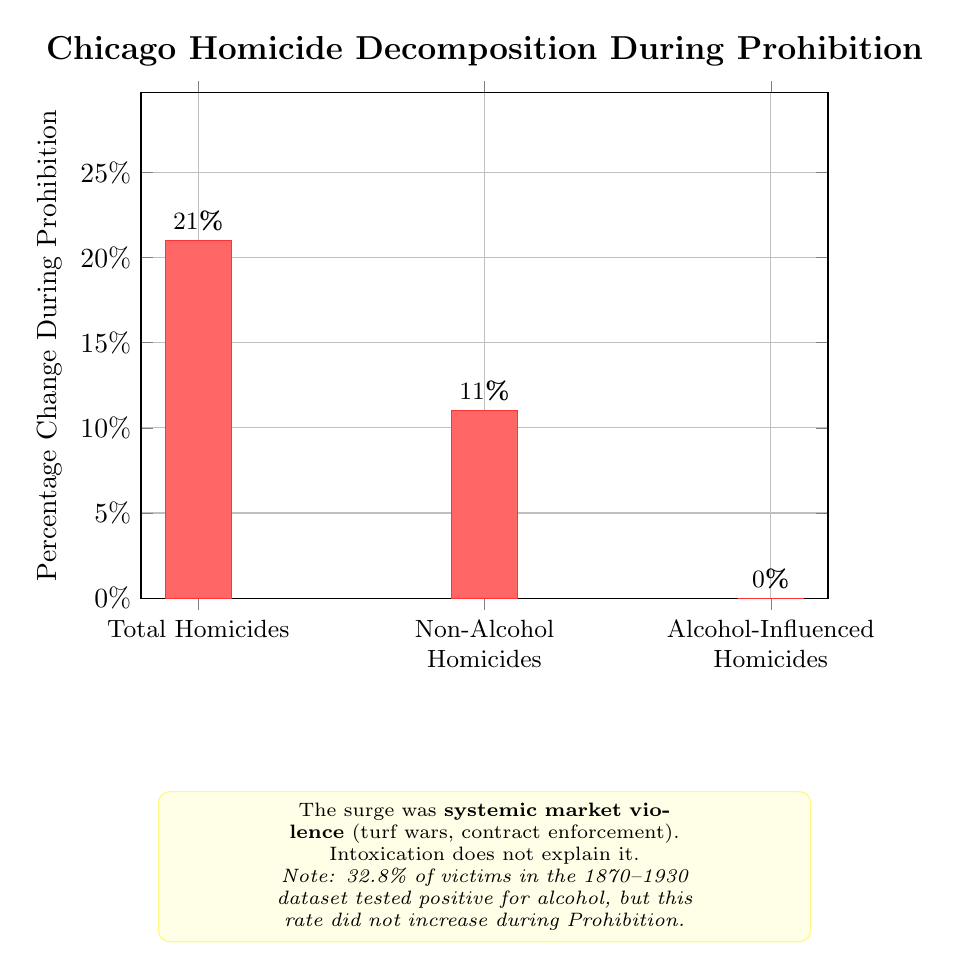
\begin{tikzpicture}
\begin{axis}[
    ybar,
    bar width=24pt,
    width=0.85\textwidth,
    height=8cm,
    ylabel={Percentage Change During Prohibition},
    symbolic x coords={Total Homicides,Non-Alcohol Homicides,Alcohol-Influenced Homicides},
    xtick=data,
    x tick label style={text width=3cm, align=center, font=\small},
    ymin=0, ymax=28,
    enlarge y limits={value=0.06, upper},
    nodes near coords={\pgfmathprintnumber\pgfplotspointmeta\%},
    every node near coord/.append style={font=\small\bfseries},
    grid=major,
    title={\textbf{Chicago Homicide Decomposition During Prohibition}},
    title style={font=\large},
    ytick={0,5,10,15,20,25},
    yticklabel={\pgfmathprintnumber\tick\%},
]
\addplot[fill=red!60, draw=red!80] coordinates {
(Total Homicides,21)
(Non-Alcohol Homicides,11)
(Alcohol-Influenced Homicides,0)
};
\end{axis}
\node[anchor=north, text width=8cm, align=center, font=\scriptsize, fill=yellow!10, draw=yellow!50, rounded corners, inner sep=4pt] at ([yshift=-2.45cm]current axis.south) {The surge was \textbf{systemic market violence} (turf wars, contract enforcement).\\Intoxication does not explain it.\\\textit{Note: 32.8\% of victims in the 1870--1930 dataset tested positive for alcohol, but this rate did not increase during Prohibition.}};
\end{tikzpicture}
\caption{Decomposition of the Prohibition-era homicide increase in Chicago (1870--1930 dataset, 11,018 cases). The 21\% total increase was driven entirely by systemic market violence between rival bootlegging factions, while alcohol-influenced homicides remained unchanged---proving the violence was a structural output of the illicit market. Source: Asbridge \& Weerasinghe (2009).}
\label{fig:chicago-decomposition}
\end{figure}

Public health data corroborates. In New Orleans, despite Prohibition enforcement, the death rate from liver cirrhosis \textit{rose} by 25.1 percent between 1920 and 1929---indicating that massive quantities of toxic illicit alcohol were still being consumed \cite{homicide_mortality}. When Prohibition ended in 1933, the cirrhosis death rate plummeted by 34.7 percent over the next decade as the market re-regulated, mirroring the simultaneous collapse in the national homicide rate. The ``noble experiment'' poisoned consumption.

\paragraph{The Dual-Era Proof: Identical Algorithms, Identical Outputs.}
The algorithmic isomorphism between the two prohibition eras becomes undeniable when their homicide trajectories are overlaid on a common timeline. Both eras are aligned at their respective pre-prohibition baselines (1910 and 1960). Both trajectories peak at approximately \textbf{9.8 homicides per 100,000}---the identical lethal zenith---before declining only when the underlying market dynamics shifted (repeal of Prohibition; natural waning of crack markets). The substances changed; the architecture produced the same output to the same decimal place.

\begin{figure}[htbp]
\centering
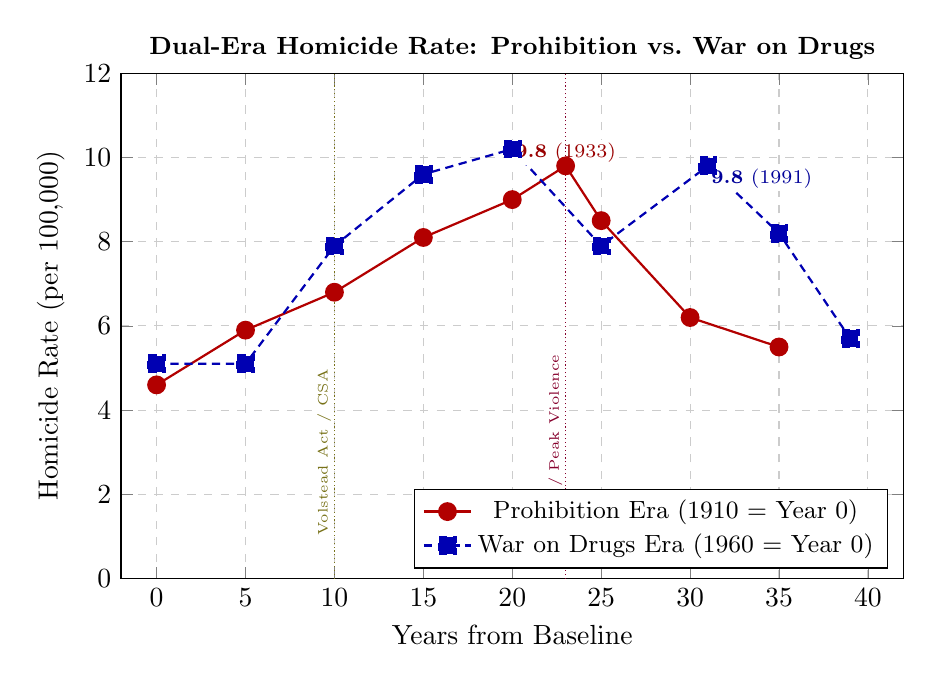
\begin{tikzpicture}
\begin{axis}[
    width=0.95\textwidth,
    height=8cm,
    title={\textbf{Dual-Era Homicide Rate: Prohibition vs.\ War on Drugs}},
    xlabel={Years from Baseline},
    ylabel={Homicide Rate (per 100{,}000)},
    xmin=-2, xmax=42,
    ymin=0, ymax=12,
    xtick={0,5,10,15,20,25,30,35,40},
    ytick={0,2,4,6,8,10,12},
    grid=major,
    grid style={dashed, gray!40},
    mark size=3pt,
    every axis title/.style={font=\bfseries\small, at={(0.5,1.05)}},
    legend style={at={(0.98,0.02)}, anchor=south east, font=\small},
]
\addplot[thick, red!70!black, mark=*] coordinates {
    (0, 4.6) (5, 5.9) (10, 6.8) (15, 8.1) (20, 9.0) (23, 9.8) (25, 8.5) (30, 6.2) (35, 5.5)
};
\addlegendentry{Prohibition Era (1910 = Year 0)}
\addplot[thick, blue!70!black, mark=square*, densely dashed] coordinates {
    (0, 5.1) (5, 5.1) (10, 7.9) (15, 9.6) (20, 10.2) (25, 7.9) (31, 9.8) (35, 8.2) (39, 5.7)
};
\addlegendentry{War on Drugs Era (1960 = Year 0)}
\node[above, font=\scriptsize, red!60!black, fill=white, inner sep=1pt] at (axis cs:23,9.8) {\textbf{9.8} (1933)};
\node[below right, font=\scriptsize, blue!60!black, fill=white, inner sep=1pt] at (axis cs:31,9.8) {\textbf{9.8} (1991)};
\draw[densely dotted, olive!80!black] (axis cs:10,0) -- (axis cs:10,12);
\node[rotate=90, anchor=south, font=\tiny, olive!80!black, fill=white, inner sep=1pt] at (axis cs:10,3) {Volstead Act / CSA};
\draw[densely dotted, purple!70!black] (axis cs:23,0) -- (axis cs:23,12);
\node[rotate=90, anchor=south, font=\tiny, purple!70!black, fill=white, inner sep=1pt] at (axis cs:23,3) {Repeal / Peak Violence};
\end{axis}
\end{tikzpicture}
\caption{\textbf{The Algorithm Is Pharmacologically Invariant.} Both prohibition eras are aligned at their pre-prohibition baselines. Both trajectories peak at 9.8 homicides per 100,000---the identical lethal zenith. The convergence is the mathematical output of the same algorithm ($P_{\text{uppet}}$ criminalizes inelastic demand $\rightarrow$ illicit market forms $\rightarrow$ competitive violence surges $\rightarrow$ $E$ harvests the terror). The substances change; the extraction kernel runs the same code. Sources: U.S.\ Vital Statistics; Bureau of the Census; FBI UCR.}
\label{fig:dual_era_homicide}
\end{figure}

The carceral state expansion that followed each era was equally parallel---but the War on Drugs apparatus exceeded its Prohibition-era predecessor by an order of magnitude:

\begin{figure}[htbp]
\centering
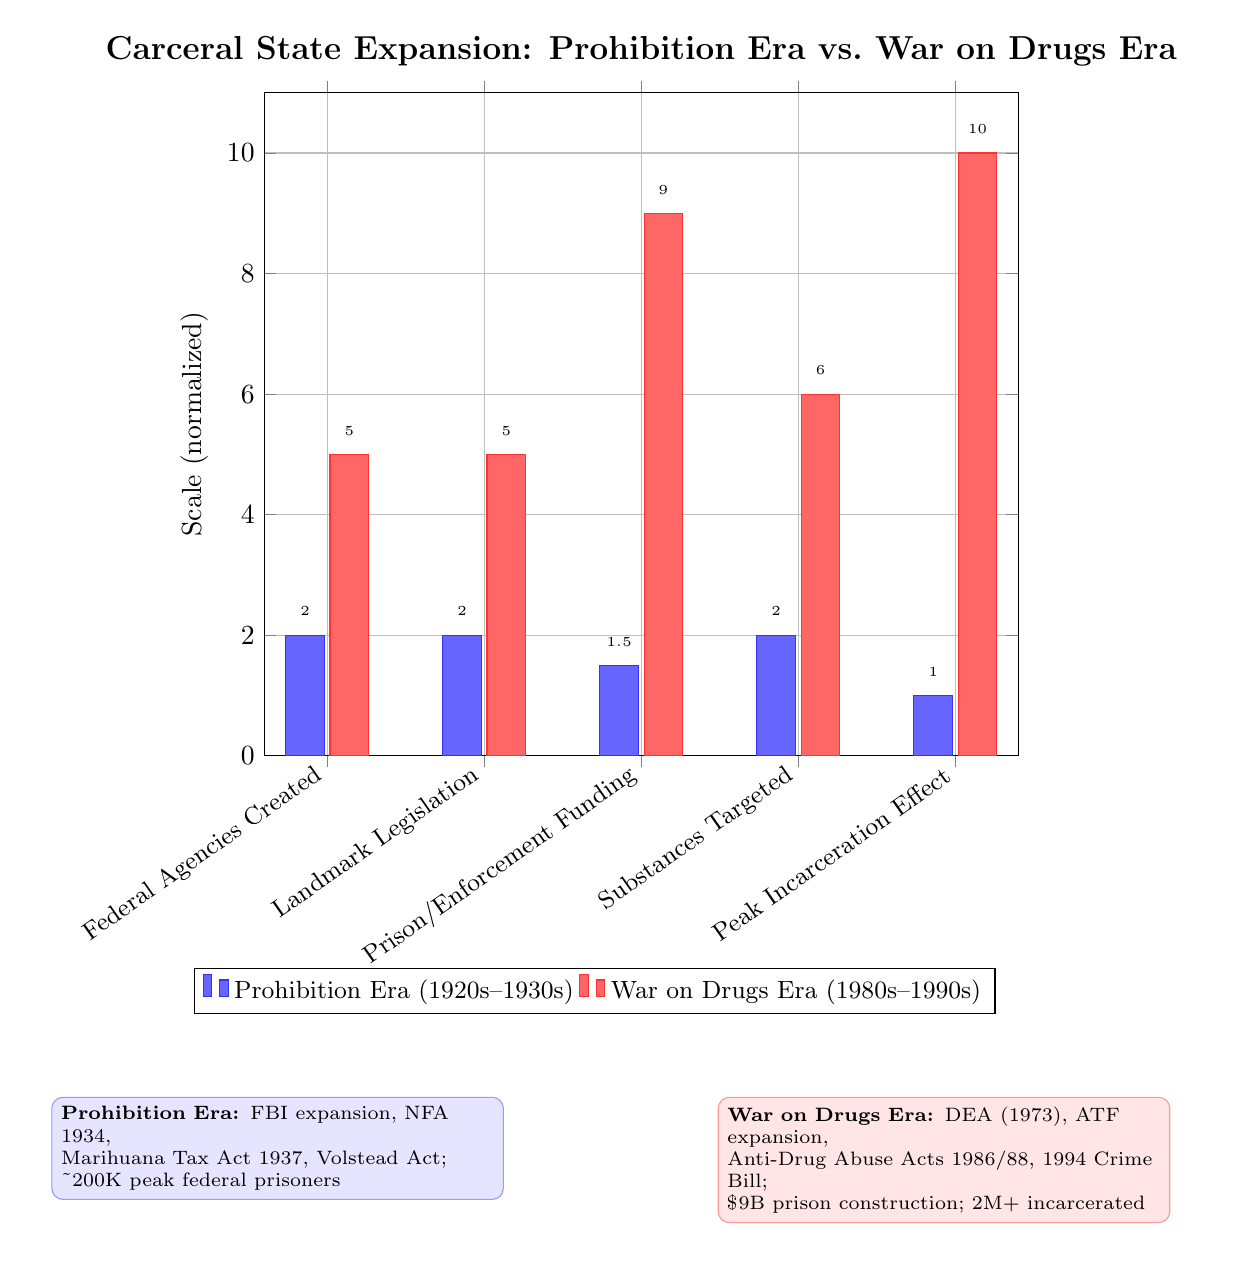
\begin{tikzpicture}
\begin{axis}[
    ybar,
    bar width=14pt,
    width=0.92\textwidth,
    height=10cm,
    clip=false,
    ylabel={Scale (normalized)},
    symbolic x coords={Federal Agencies Created,Landmark Legislation,Prison/Enforcement Funding,Substances Targeted,Peak Incarceration Effect},
    xtick=data,
    x tick label style={rotate=35, anchor=east, font=\small},
    ymin=0, ymax=11,
    legend style={at={(0.97,-0.32)}, anchor=north east, legend columns=2, font=\small},
    nodes near coords,
    every node near coord/.append style={font=\tiny, yshift=0.12cm},
    grid=major,
    title={\textbf{Carceral State Expansion: Prohibition Era vs.\ War on Drugs Era}},
    title style={font=\large},
]
\addplot[fill=blue!60, draw=blue!80] coordinates {
(Federal Agencies Created,2)
(Landmark Legislation,2)
(Prison/Enforcement Funding,1.5)
(Substances Targeted,2)
(Peak Incarceration Effect,1)
};
\addplot[fill=red!60, draw=red!80] coordinates {
(Federal Agencies Created,5)
(Landmark Legislation,5)
(Prison/Enforcement Funding,9)
(Substances Targeted,6)
(Peak Incarceration Effect,10)
};
\legend{Prohibition Era (1920s--1930s), War on Drugs Era (1980s--1990s)}
\end{axis}
\node[anchor=north west, font=\scriptsize, text width=5.5cm, fill=blue!10, draw=blue!40, rounded corners] at ([xshift=-0.2cm, yshift=-1.05cm]current axis.outer south west) {
\textbf{Prohibition Era:} FBI expansion, NFA 1934,\\
Marihuana Tax Act 1937, Volstead Act;\\
\textasciitilde 200K peak federal prisoners
};
\node[anchor=north east, font=\scriptsize, text width=5.5cm, fill=red!10, draw=red!40, rounded corners] at ([xshift=-0.2cm, yshift=-1.05cm]current axis.outer south east) {
\textbf{War on Drugs Era:} DEA (1973), ATF expansion,\\
Anti-Drug Abuse Acts 1986/88, 1994 Crime Bill;\\
\$9B prison construction; 2M+ incarcerated
};
\path ([xshift=-0.5cm,yshift=-2.85cm]current axis.outer south west)
      ([xshift=0.5cm,yshift=-2.85cm]current axis.outer south east);
\end{tikzpicture}
\caption{\textbf{The Carceral Ratchet: Each Prohibition Cycle Expands $F_{\text{enforce}}$ Permanently.} Normalized scale: 1 = Prohibition-era baseline, 10 = War on Drugs peak. The algorithm's output scales with each execution: the second cycle produced 10$\times$ the incarceration infrastructure of the first. The ratchet locks in one direction---the NFA was never repealed, the DEA was never dissolved, the prison infrastructure was never decommissioned. Each manufactured crisis leaves behind permanent institutional architecture. Sources: BJS; DOJ budget records; Mauer (2006); Alexander (2010).}
\label{fig:carceral_expansion_comparison}
\end{figure}
\FloatBarrier

\subsubsection{The Enforcement Asymmetry: $F_{\text{enforce}}$ by Design}

The inability of the state to curb the rising violence was a structural asymmetry so grotesque that it raises the question of whether $F_{\text{enforce}}$ was designed to succeed at all---or whether it was designed to fail visibly enough to justify its own expansion \cite{mobmuseum_agents}.

The Volstead Act tasked the Treasury Department's Prohibition Unit with policing the entire geography of the United States---12,000 miles of shoreline, 3,900 miles of international border---with a meager force of 1,500 agents. In 1923, the combined federal and state enforcement budget was less than \$500,000. Agent salaries ranged from \$1,200 to \$3,000 annually. Meanwhile, a single syndicate---Capone's Outfit---was generating \$100 million per year and distributing \$500,000 per month in bribes. By 1930, 1,587 federal Prohibition employees had been terminated for offenses including perjury, robbery, bribery, and embezzlement \cite{fjc_prohibition, mobmuseum_agents}.

\begin{figure}[htbp]
\centering
\hspace*{-0.04\textwidth}%
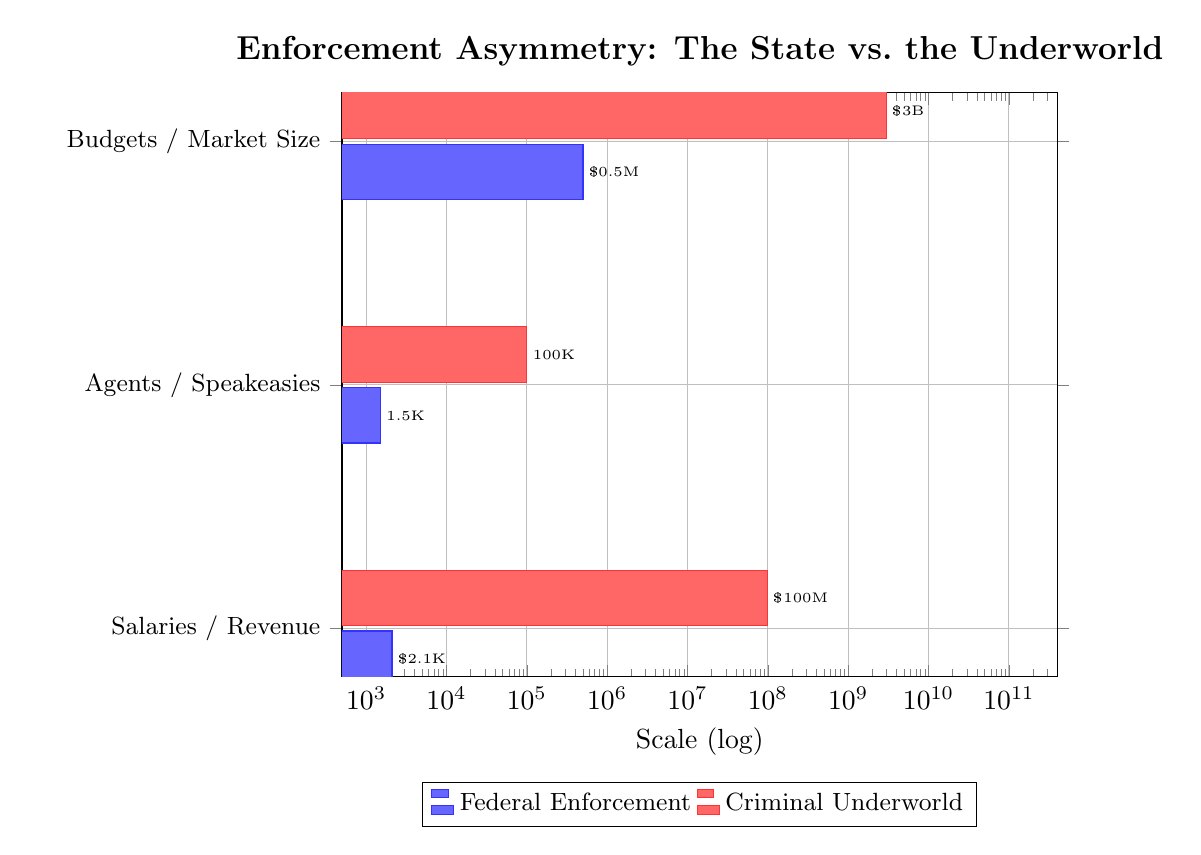
\begin{tikzpicture}
\begin{axis}[
    xbar,
    bar width=20pt,
    width=0.88\textwidth,
    height=9cm,
    xlabel={Scale (log)},
    xmode=log,
    xmin=500, xmax=10000000000,
    enlarge x limits={0.22, upper},
    symbolic y coords={Salaries / Revenue,Agents / Speakeasies,Budgets / Market Size},
    ytick=data,
    y tick label style={font=\small, text width=3.6cm, align=right},
    nodes near coords,
    every node near coord/.append style={font=\tiny, anchor=west, inner xsep=2pt},
    point meta=explicit symbolic,
    grid=major,
    title={\textbf{Enforcement Asymmetry: The State vs.\ the Underworld}},
    title style={font=\large},
    legend style={at={(0.5,-0.18)}, anchor=north, legend columns=2, font=\small},
]
\addplot[fill=blue!60, draw=blue!80] coordinates {
(2100,Salaries / Revenue) [\$2.1K]
(1500,Agents / Speakeasies) [1.5K]
(500000,Budgets / Market Size) [\$0.5M]
};
\addplot[fill=red!60, draw=red!80] coordinates {
(100000000,Salaries / Revenue) [\$100M]
(100000,Agents / Speakeasies) [100K]
(3000000000,Budgets / Market Size) [\$3B]
};
\legend{Federal Enforcement, Criminal Underworld}
\end{axis}
\end{tikzpicture}
\caption{The structural asymmetry between federal enforcement resources and the scale of the illicit alcohol economy. With 1,500 agents earning \$1,200--\$3,000 annually against an underground economy generating over \$100 million annually for a single syndicate, $F_{\text{enforce}}$ was outmatched by multiple orders of magnitude. The asymmetry was the architecture functioning as designed---visible failure justifying permanent expansion.}
\label{fig:enforcement-asymmetry}
\end{figure}

The framework reads this asymmetry as structural. The system deployed 1,500 agents against a \$3 billion underground economy---the same system that had just mobilized four million soldiers for a world war. The state that could project military force across the Atlantic could not police its own coastline. The enforcement apparatus was designed to \textit{demonstrate the impossibility of local enforcement}---creating the political case for permanent federal police expansion. When direct enforcement failed, the government pivoted: the Treasury Department's Special Intelligence Unit, led by Elmer Irey, prosecuted Capone for felony tax evasion, sidestepping bootlegging and murder charges \cite{fbi_gangster}. The system could not beat the syndicates in the streets, so it attacked them through the financial infrastructure---the same tax code it would subsequently weaponize in the NFA and the Marihuana Tax Act of 1937.

\subsubsection{The St.\ Valentine's Day Massacre: The Interface Shift}

The statistics document the macro-level tragedy. The political shift that enabled the NFA was driven by a single spectacular act of public violence---the same pattern the framework documents in the post-assassination gun control of 1968 (GCA) and the post-mass-shooting legislation of subsequent decades. The system requires a \textit{visible atrocity} to convert diffuse public anxiety into concentrated political capital.

On the morning of February 14, 1929, four men---two dressed in stolen Chicago Police Department uniforms---entered a garage at 2122 N. Clark Street, where seven members of George ``Bugs'' Moran's North Side Gang had been lured under the pretense of receiving a hijacked whiskey shipment \cite{wikipedia_valentine, chicago_valentine, michiganology_valentine}. The executioners ordered the men to line up against the rear brick wall and unleashed 70 rounds from two Thompson submachine guns and two shotguns into their backs and heads. Moran himself narrowly escaped, having arrived late. Capone, vacationing in Florida with a carefully constructed alibi, was universally recognized as the architect but never prosecuted for the massacre.

The St.\ Valentine's Day Massacre operated as what the framework terms an \textbf{interface shift}. Before 1929, much of the American public viewed bootleggers as romanticized, anti-establishment figures providing a desired service in defiance of an unpopular law. The sheer barbarity of the garage executions---captured in gruesome press photographs disseminated nationally---evaporated this public sympathy overnight. The massacre forced the federal government to acknowledge that municipal police forces were entirely outgunned and hopelessly corrupted, necessitating a federalized response \cite{poynter_valentine, natgeo_machinegun}. Map this onto the framework: the system required the public to \textit{see} the violence---to experience it as a media spectacle---before the violence could be converted into legislative capital. The algorithm's Step~4 (Public Panic) is an \textit{engineered psychological operation} in which the spectacle of violence is curated, amplified, and directed toward a predetermined legislative outcome.

\subsubsection{The Legislative Architecture: Taxation as Regulation}

The extreme violence of the Prohibition era provided the federal state with the political leverage to construct the foundational architecture of modern American gun control \cite{nfa1934, atf_nfa}.

The signature weapon of the era was the Thompson submachine gun---invented by John T.\ Thompson in 1918 for trench warfare, firing .45 ACP ammunition at 600 to 900 rounds per minute \cite{wikipedia_thompson}. Equipped with 50- or 100-round drum magazines and easily concealable beneath a topcoat, the weapon provided squad-level automatic firepower to single individuals. Because it was legally available for commercial purchase, it was rapidly adopted by syndicates and bank robbers, earning the moniker ``Chicago Typewriter.''

As the homicide rate climbed to its 1933 peak, and following an assassination attempt on President-elect Roosevelt, the newly formed administration declared a national ``War on Crime'' \cite{fbi_gangster, pbs_gangsters}. Attorney General Homer S.\ Cummings recognized that local ordinances were insufficient against heavily armed, interstate cartels and drafted what would become the National Firearms Act of 1934---the first comprehensive federal firearm legislation in U.S. history.

The constitutional strategy was profoundly shaped by the constraints of the era. In the 1930s, strict limits on the Commerce Clause posed significant barriers to an outright federal firearms ban. To circumvent this, Cummings utilized Congress's enumerated Article~I power to levy taxes \cite{cornell_nfa, fulbright_nfa}. During testimony before the House Committee on Ways and Means, Cummings explicitly admitted the legislative sleight-of-hand:

\begin{quote}
``If we had a statute absolutely forbidding any human being to have a machine gun, you might say there is some constitutional question involved. But when you say, `we will tax the machine gun,' \ldots{} you are easily within the law.'' \cite{cornell_nfa}
\end{quote}

The admission is structurally significant. The Attorney General of the United States confessed, on the congressional record, that the NFA was a \textit{prohibition disguised as a tax} to evade constitutional review. The system priced the weapons out of existence. The original draft (H.R. 9066) sought to impose registration and heavy taxation on \textit{all} concealable firearms, including standard pistols and revolvers. Intense lobbying by the NRA forced a critical compromise: handguns were stripped from the final legislation \cite{recoil_nfa, ebsco_nfa}.

{\def\LTcaptype{none}
\begin{longtable}[]{@{}
  >{\raggedright\arraybackslash}p{0.20\linewidth}
  >{\raggedright\arraybackslash}p{0.25\linewidth}
  >{\raggedright\arraybackslash}p{0.25\linewidth}
  >{\raggedright\arraybackslash}p{0.25\linewidth}@{}}
\toprule
Firearm Category & Definition Parameters & Regulatory Action & Purpose / Target Demographic \\
\midrule
\endhead
\bottomrule
\endlastfoot
\textbf{Machine Guns} & Any weapon shooting automatically more than one shot without manual reloading. & \$200 Tax + Registration & Target cartel enforcers (Thompson SMG). \\
\textbf{Short-Barreled Shotguns} & Shotgun having a barrel less than 18 inches in length. & \$200 Tax + Registration & Target easily concealable bank robbery tools. \\
\textbf{Short-Barreled Rifles} & Rifle having a barrel less than 16 inches in length. & \$200 Tax + Registration & Target easily concealable long guns. \\
\textbf{Silencers/Mufflers} & Device for silencing, muffling, or diminishing the report of a portable firearm. & \$200 Tax + Registration & Target assassination tools used by hitmen. \\
\textbf{Pistols/Revolvers} & Standard handguns. & \emph{Removed from Bill} & Originally targeted; removed via NRA lobbying. \\
\end{longtable}
}

The finalized NFA imposed a \$200 transfer and making tax on machine guns, short-barreled rifles and shotguns, and silencers \cite{nfa1934}. In 1934 dollars, \$200 was equivalent to approximately \$4,800 in 2026 purchasing power---the price of a used car \cite{blscpi}. When a brand-new Thompson submachine gun cost approximately \$175, the \$200 tax effectively doubled the weapon's cost. For a \$25 sawed-off shotgun, the tax represented an 800 percent price increase. This was a \textit{price-out-of-existence} mechanism designed to make the most effective military hardware economically inaccessible to the working class; revenue generation was incidental.

\begin{figure}[htbp]
\centering
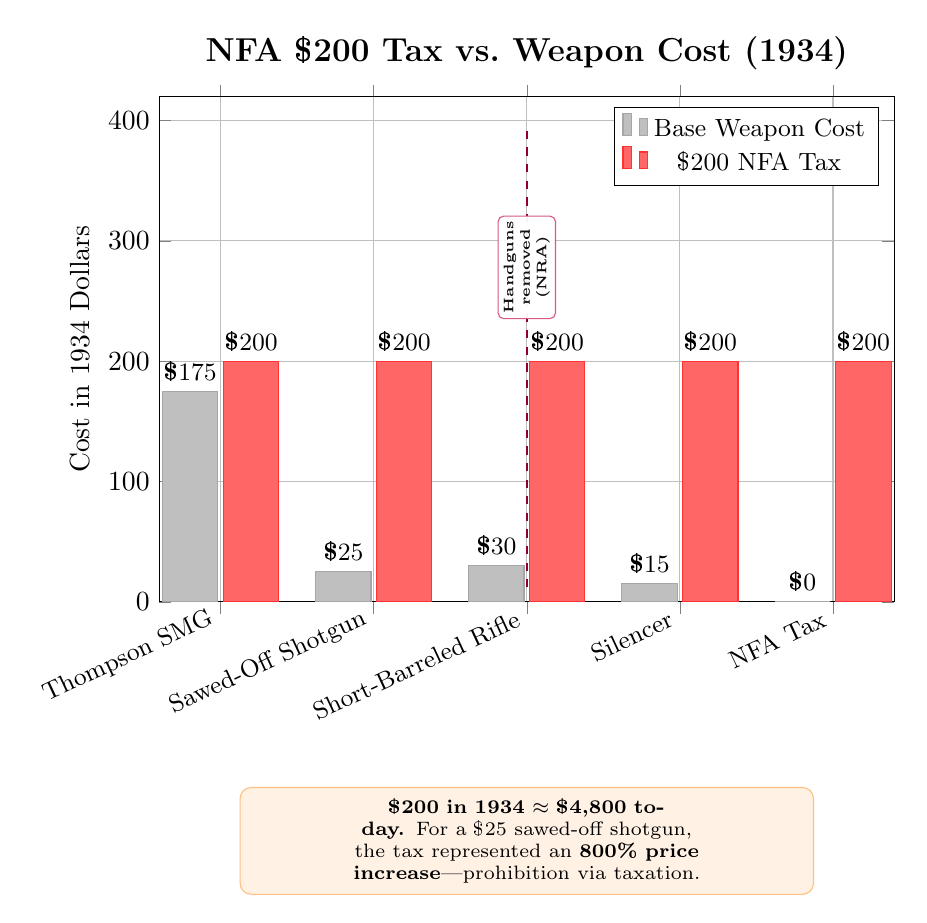
\begin{tikzpicture}
\begin{axis}[
    ybar,
    bar width=20pt,
    width=0.9\textwidth,
    height=8cm,
    ylabel={Cost in 1934 Dollars},
    symbolic x coords={Thompson SMG,Sawed-Off Shotgun,Short-Barreled Rifle,Silencer,NFA Tax},
    xtick=data,
    x tick label style={rotate=25, anchor=east, font=\small},
    ymin=0, ymax=420,
    nodes near coords={\$\pgfmathprintnumber\pgfplotspointmeta},
    every node near coord/.append style={font=\small\bfseries},
    grid=major,
    title={\textbf{NFA \$200 Tax vs.\ Weapon Cost (1934)}},
    title style={font=\large},
    legend style={at={(0.98,0.98)}, anchor=north east, font=\small},
]
\addplot[fill=gray!50, draw=gray!70] coordinates {
(Thompson SMG,175)
(Sawed-Off Shotgun,25)
(Short-Barreled Rifle,30)
(Silencer,15)
(NFA Tax,0)
};
\addplot[fill=red!60, draw=red!80] coordinates {
(Thompson SMG,200)
(Sawed-Off Shotgun,200)
(Short-Barreled Rifle,200)
(Silencer,200)
(NFA Tax,200)
};
\legend{Base Weapon Cost, \$200 NFA Tax}
\pgfplotsextra{%
  \draw[dashed, purple!75!black, line width=0.9pt] (axis cs:{Short-Barreled Rifle},12) -- (axis cs:{Short-Barreled Rifle},398);
  \node[rotate=90, anchor=center, font=\tiny\bfseries, text=black, fill=white, fill opacity=0.94, draw=purple!65, rounded corners=2pt, inner sep=2pt, align=center] at (axis cs:{Short-Barreled Rifle},278) {Handguns\\removed\\(NRA)};
}
\end{axis}
\node[anchor=north, text width=7cm, align=center, font=\scriptsize, fill=orange!10, draw=orange!50, rounded corners, inner sep=4pt] at ([yshift=-2.35cm]current axis.south) {\textbf{\$200 in 1934 $\approx$ \$4,800 today.} For a \$25 sawed-off shotgun,\\the tax represented an \textbf{800\% price increase}---prohibition via taxation.};
\end{tikzpicture}
\caption[The NFA Transfer Tax]{The NFA's \$200 transfer tax shown against the base cost of each regulated weapon category. The tax doubled the cost of a Thompson submachine gun and increased the cost of cheaper weapons by 670--1,300\%, achieving \emph{de facto} prohibition through prohibitive pricing. Handguns were originally included but removed via NRA lobbying---the NRA's first documented intervention in the disarmament timeline.}
\label{fig:nfa-tax}
\end{figure}

Now examine the structural function through the framework. The Buffer Class ($I_{\text{buffer}}$) was persuaded to surrender its constitutional right to military-equivalent hardware in order to spite a racialized criminal Out-group---Italian-American and Jewish immigrant communities recast as the ``armed underworld.'' This is the \textit{identical dynamic} to the 1705 wages of whiteness documented in Chapter~\ref{ch:bacon}: the Buffer Class accepting a reduction in its own material position in exchange for a psychological wage of superiority over the designated Other. Capone could easily afford the \$200 tax but avoided registration to prevent providing federal agents with documented proof of his arsenal, so the gangsters remained armed. The NFA disarmed the \textit{working class}, permanently pricing military-equivalent hardware out of reach for the population most likely to need the kinetic guarantee.

The NFA's jurisprudential architecture was upheld in \textit{Sonzinsky v.\ United States} (1937), which validated the taxing mechanism, and \textit{United States v.\ Miller} (1939), which ruled that the Second Amendment did not protect weapons lacking a ``reasonable relationship to the preservation of a well-regulated militia'' \cite{dickinson_nfa, ebsco_nfa}. The success of the NFA in practically eliminating the legal commercial market for fully automatic weapons established a durable precedent. By successfully utilizing the tax code to enact sweeping social control, the Roosevelt administration set the constitutional template that would be used to draft the \textbf{Marihuana Tax Act of 1937}---launching the federal war on drugs using the \textit{exact same constitutional mechanism} \cite{cato_prohibition}. The disarmament architecture and the carceral architecture share a common constitutional root: the taxing power weaponized as prohibition.\footnote{On April 10, 2026, the Fifth Circuit Court of Appeals struck down a 158-year-old federal ban on home distilling, enacted in 1868 to prevent liquor tax evasion, as an ``unnecessary and improper'' exercise of the taxing power. The three-judge panel, led by Circuit Judge Edith H.\ Jones, held that a purported tax which eliminates the taxable activity entirely---generating zero revenue---cannot be sustained as a legitimate exercise of Congress's taxing authority (\textit{Hobby Distillers Association v.\ United States}, 5th Cir.\ 2026 \cite{hobby_distillers_2026}). The constitutional logic of that ruling applies with direct force to the NFA's \$200 transfer tax, which was deliberately calibrated to price military-equivalent hardware out of the civilian market, with revenue as an incidental feature---and to the Marihuana Tax Act of 1937, which followed the identical template. If the taxing power cannot prohibit home distilling because the prohibition produces no tax, it cannot constitutionally prohibit machine gun transfers for the same reason. \textit{Sonzinsky}'s validation of the NFA now rests on precisely the constitutional ground the Fifth Circuit has declared untenable.} The militia-nexus \textit{Miller} established to justify the NFA later becomes the first jaw of a doctrinal self-contradiction when modern state assault-weapons bans invoke the identical military character to \textit{exclude} the same category of arms---a pincer analyzed fully in Section~\ref{subsec:doctrinal_pincer}.

The \$200 tax stamp has never been adjusted for inflation. In 2026, \$200 is no longer prohibitive---which is precisely why the system has proposed updating it. Recent legislative proposals have called for a tax of \$4,709 per NFA item, transparently designed to restore the original economic barrier \cite{murphy2025nfa}. The system knows exactly what price point eliminates working-class access; it merely recalibrates the filter when inflation erodes its effectiveness.

\subsubsection{The Post-Prohibition Proof: Repeal as Controlled Experiment}

By the early 1930s, the ``noble experiment'' was universally recognized as catastrophic. The Volstead Act had birthed a multi-million-dollar criminal underworld, corrupted the judiciary, and flooded city streets with automatic weapon fire \cite{mobmuseum_repeal}. The Great Depression altered the political calculus: the federal government, desperate for tax revenue and job creation, could no longer afford to squander millions enforcing a despised law while surrendering billions in potential excise taxes to criminal cartels. In the 1932 presidential election, Roosevelt campaigned aggressively on Repeal. The Twenty-First Amendment was ratified on December 5, 1933, ending National Prohibition.

The sociological impact was immediate and undeniable. With the primary economic engine of the criminal underworld eliminated, contractual disputes over territory and supply were settled in courtrooms through civil litigation; Thompson submachine guns in alleyways were no longer the enforcement mechanism. The national homicide rate, which had peaked in 1933, underwent a dramatic, sustained reversal. Between 1933 and 1940, Detroit's homicide rate plummeted by 66.3 percent, New Orleans by 56.6 percent, New York City by 41.8 percent, and Chicago by 33.1 percent \cite{hoplofobia_prohibition, newdeal_crime}. This decline continued steadily through the 1940s and 1950s, conclusively proving that the violence of the 1920s was a direct, localized symptom of the prohibitionary market structure.

\begin{figure}[htbp]
\centering
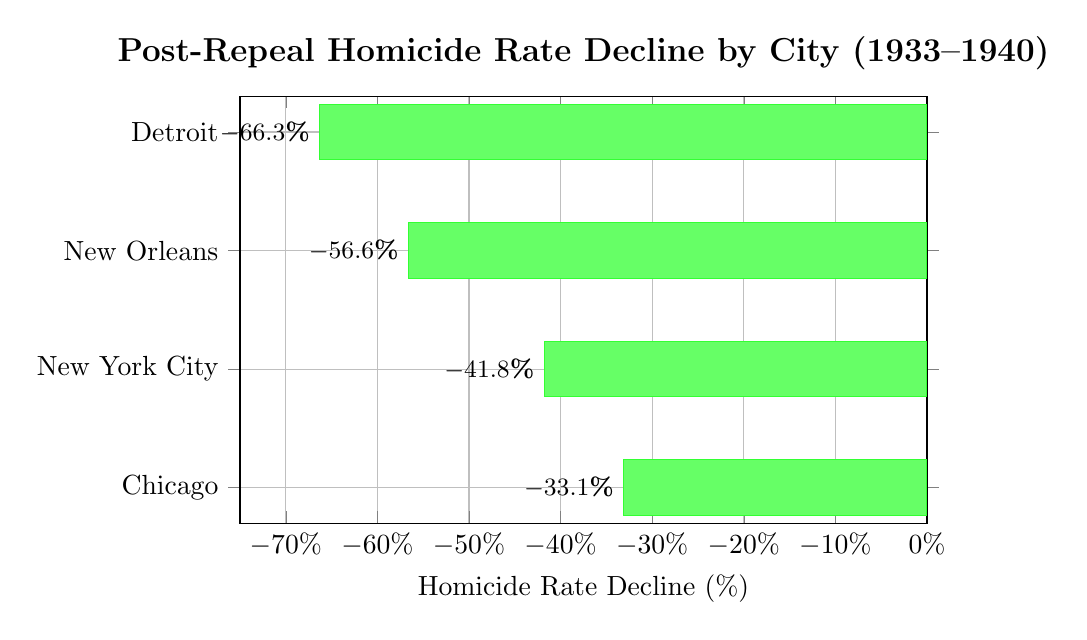
\begin{tikzpicture}
\begin{axis}[
    xbar,
    bar width=20pt,
    width=0.85\textwidth,
    height=7cm,
    xlabel={Homicide Rate Decline (\%)},
    symbolic y coords={Chicago,New York City,New Orleans,Detroit},
    ytick=data,
    y tick label style={font=\normalsize},
    xmin=-75, xmax=0,
    nodes near coords={\pgfmathprintnumber\pgfplotspointmeta\%},
    every node near coord/.append style={font=\small\bfseries, anchor=east},
    grid=major,
    title={\textbf{Post-Repeal Homicide Rate Decline by City (1933--1940)}},
    title style={font=\large},
    xticklabel={\pgfmathprintnumber\tick\%},
]
\addplot[fill=green!60, draw=green!80] coordinates {
(-33.1,Chicago)
(-41.8,New York City)
(-56.6,New Orleans)
(-66.3,Detroit)
};
\end{axis}
\end{tikzpicture}
\caption{The dramatic collapse in urban homicide rates following the repeal of Prohibition in 1933. Detroit, a primary smuggling corridor from Canada, experienced the steepest decline (66.3\%). The synchronized drop across all major cities proves the violence was a structural output of the illicit market.}
\label{fig:post-repeal-decline}
\end{figure}

Read this as a controlled experiment. When the state removed the prohibition, the violence collapsed. When the state reimposed prohibition sixty years later---this time targeting cocaine and crack---the violence returned with identical characteristics: the same turf wars, the same market-driven homicide surge, the same racialized populations bearing the burden of the violence, the same political class harvesting the crisis to expand $F_{\text{enforce}}$ and contract the kinetic guarantee. The 1994 Crime Bill is the NFA's grandchild---born from the same algorithm, justified by the same manufactured crisis, serving the same extraction kernel.

The organizational infrastructure Prohibition created adapted as the violence receded. The massive capital amassed during the 1920s provided mob bosses like Meyer Lansky, Frank Costello, and the leaders of the Chicago Outfit with the resources to transition into illegal gambling, labor union racketeering, and the international narcotics trade \cite{pbs_gangsters}. Former rum-running fleets were repurposed for smuggling heroin and cocaine. The wealth accumulated from bootlegging was invested in the legal casino industry in Las Vegas. Prohibition \textit{corporatized} the American Mafia, providing the organizational blueprint and financial war chest that sustained illicit operations for the next half-century.

Simultaneously, the federal law enforcement apparatus expanded to fight bootleggers---the FBI under Hoover, the Treasury Department's Intelligence Units under Irey---retained their enhanced budgets, personnel, and statutory authority after Repeal \cite{fbi_gangster}. The bureaucratic infrastructure built to wage the ``War on Crime'' became a permanent fixture, fundamentally shifting the balance of police power from local municipalities to the federal government. $F_{\text{enforce}}$ expanded during the crisis and \textit{never contracted when the crisis ended}. This is the ratchet mechanism: each manufactured crisis permanently expands the enforcement apparatus, and no amount of post-crisis normalization reverses the expansion.

\begin{figure}[htbp]
\centering
\begin{tikzpicture}[
    node distance=1cm and 0.6cm,
    every node/.style={font=\small},
    phase/.style={rectangle, draw=#1!70, fill=#1!12, text width=3cm, align=center, rounded corners, minimum height=1cm},
    cycle/.style={-{Stealth[length=3mm]}, ultra thick, gray!60},
    era/.style={rectangle, draw=#1!80, fill=#1!20, text width=3.2cm, align=center, rounded corners, minimum height=0.8cm, font=\scriptsize},
]
\node[phase=red] (prohibit) {\textbf{1. State Prohibition}\\Criminalize inelastic demand};
\node[phase=orange, right=1.5cm of prohibit] (market) {\textbf{2. Illicit Market}\\Black market forms};
\node[phase=red!80!black, below=1.5cm of market] (violence) {\textbf{3. Market Violence}\\Lethal turf wars};
\node[phase=purple, left=1.5cm of violence] (panic) {\textbf{4. Public Panic}\\Media \& political crisis};
\node[phase=blue, below=1.5cm of panic] (expand) {\textbf{5. State Expansion}\\New federal authority};
\draw[cycle] (prohibit) -- (market);
\draw[cycle] (market) -- (violence);
\draw[cycle] (violence) -- (panic);
\draw[cycle] (panic) -- (expand);
\draw[cycle, bend left=40] (expand) to node[midway, left, font=\scriptsize, text width=2cm, align=center] {Cycle repeats\\with new substance} (prohibit);
\node[era=blue, left=0.3cm of prohibit, yshift=1.5cm] (e1a) {Volstead Act\\(1920)};
\node[era=blue, right=0.3cm of market, yshift=1.5cm] (e1b) {Bootlegging\\Rum Row};
\node[era=blue, right=0.3cm of violence] (e1c) {Gang Wars\\St.\ Valentine's};
\node[era=blue, left=0.3cm of panic] (e1d) {``War on Crime''};
\node[era=blue, below left=0.3cm and 0.3cm of expand] (e1e) {NFA 1934\\FBI Expansion};
\node[era=red, right=0.3cm of prohibit, yshift=1.5cm] (e2a) {CSA / War\\on Drugs};
\node[era=red, right=0.3cm of market, yshift=0.7cm] (e2b) {Crack Trade\\Drug Cartels};
\node[era=red, right=0.3cm of violence, yshift=-0.8cm] (e2c) {Crack Epidemic\\Homicide Surge};
\node[era=red, left=0.3cm of panic, yshift=-0.8cm] (e2d) {``Superpredator''\\Panic};
\node[era=red, below right=0.3cm and 0.3cm of expand] (e2e) {1994 Crime Bill\\DEA / \$9B Prisons};
\node[font=\bfseries\footnotesize, blue!70] at ([yshift=2.3cm]prohibit.north) {1920s Era};
\node[font=\bfseries\footnotesize, red!70] at ([yshift=2.3cm, xshift=3.5cm]prohibit.north) {1980s Era};
\end{tikzpicture}
\caption{The recurring state algorithm identified across both prohibition eras. The state criminalizes inelastic demand, generating a violent black market, then leverages that violence to permanently expand federal police authority. The 1920s Alcohol Prohibition $\rightarrow$ NFA/FBI cycle was replicated precisely by the War on Drugs $\rightarrow$ 1994 Crime Bill/DEA cycle sixty years later. The cycle is self-reinforcing: expanded authority enables further prohibition, which generates further violence.}
\label{fig:prohibition-algorithm}
\end{figure}

\begin{keyinsight}[The Prohibition--Crack Isomorphism]
The Prohibition era and the crack era are \textit{isomorphic executions of the same algorithm}. Change the prohibited commodity (alcohol $\rightarrow$ cocaine), change the racialized population blamed for the violence (Italian/Jewish immigrants $\rightarrow$ Black Americans), keep the five-step cycle identical, and observe the identical legislative output: permanent expansion of $F_{\text{enforce}}$, permanent contraction of the kinetic guarantee, permanent expansion of the carceral state. The NFA (1934) and the Violent Crime Control Act (1994) are the same function evaluated at two different inputs. The algorithm is substance-invariant.
\end{keyinsight}

\subsubsection{The \$0 Tax Paradox: A Source-Code Attack on the NFA}

In 2025, Congress reduced the NFA tax on suppressors and short-barreled rifles to \$0---effectively eliminating the economic filter that had gated access to these categories of arms for 91 years \cite{nfataxzero}. This legislative act created a constitutional paradox that the framework identifies as the most significant threat to the NFA's existence since its enactment.

The paradox is structural. The NFA was enacted exclusively under Congress's taxing power---the specific constitutional authority to levy taxes. The Supreme Court upheld the NFA in \textit{Sonzinsky v.\ United States} (1937) on precisely this basis: the \$200 tax was a valid exercise of the taxing power, and the registration requirements were merely incidental to its administration. But if the tax is \$0, there is no tax. And if there is no tax, the constitutional foundation that justified the entire regulatory apparatus---the registration, the wait times, the background checks, the felony penalties for non-compliance---disappears.

Litigants have recognized this vulnerability and are executing what the framework terms a \textbf{source-code attack}: they are attacking the \textit{constitutional root} of the statute itself, bypassing challenges to the NFA's day-to-day enforcement and arguments that the ATF exercises too much discretion. The argument is precise: a law enacted under the taxing power cannot survive the elimination of the tax. The registration and restriction system that remains is a regulatory apparatus without a constitutional anchor \cite{nfataxzero}.

The government's response reveals the Interface Swap in real time. The Department of Justice, recognizing that the taxing power justification has collapsed, has attempted to retroactively recharacterize the NFA as an exercise of the Commerce Clause---keeping the restriction mechanism (the kernel) intact while swapping the legal justification (the interface). The plaintiffs have blocked this maneuver by arguing that courts cannot retroactively rewrite a statute's constitutional basis after the fact: if Congress enacted the NFA under the taxing power, the judiciary cannot rescue it by inventing a Commerce Clause justification that Congress never invoked.

Read this through the framework's variable hierarchy: the \$200 tax was the original proxy variable ($P_{\text{economic}}$) that transformed the Second Amendment from a universal right into a class-gated privilege. Congress's reduction of the tax to \$0 left the NFA's registration and restriction architecture intact while eliminating the \textit{constitutional basis} for that architecture. The system now faces a binary: either restore the economic filter (the proposed \$4,709 tax), or watch the NFA's constitutional foundation dissolve under its own logic. The Elite built the disarmament architecture on a taxing power foundation; the population is now using the system's own rules to pull out the foundation and let the structure collapse.

If the source-code attack succeeds, the implications cascade through the entire disarmament timeline. The NFA is the foundational layer of federal firearms regulation---the GCA (1968), FOPA (1986), and Brady Act (1993) all build upon or reference its regulatory framework. Dismantling the NFA's constitutional basis threatens the structural integrity of every subsequent layer of federal disarmament legislation that assumed the NFA's validity as a given.

\FloatBarrier

\subsection{The Mulford Act (1967): The Pristine Proof}
\label{sec:mulford}

If the framework required a single piece of evidence to prove that gun control functions as an extraction-kernel mechanism, the Mulford Act would be that evidence.

In 1966, the Black Panther Party for Self-Defense was founded in Oakland, California, with an explicit operational mandate: armed citizens would monitor the Enforcement Class ($F_{\text{enforce}}$)---the Oakland Police Department---during interactions with members of $O_{\text{racialized}}$. The Panthers exercised their legal right to openly carry loaded firearms in public, creating a visible, organized kinetic counterbalance to police power \cite{bloom2013, mulford1967}.

The system's response was instantaneous. Republican Governor Ronald Reagan, with the active support of the National Rifle Association, signed the Mulford Act in 1967, banning the open carry of loaded firearms in California. Reagan---who would later be canonized as the patron saint of conservative gun rights---told reporters: ``There is absolutely no reason why out on the street today a civilian should be carrying a loaded weapon'' \cite{winkler2011}. He said this \textit{exclusively} in response to armed Black citizens.

Map this onto the framework:

\begin{enumerate}
    \item $O_{\text{racialized}}$ achieves visible lethal parity with $F_{\text{enforce}}$ through legal exercise of the kinetic guarantee.
    \item The system detects a threat to the inequality $L_E \gg L_O$.
    \item The system \textit{rewrites the rules} to restore the asymmetry, creating new law that eliminates the legal basis for the Out-group's kinetic capacity.
    \item The rewrite is supported by the NRA and the Republican Party---the very institutions that publicly claim to defend the Second Amendment.
\end{enumerate}

The Mulford Act proves that ``gun rights'' and ``gun control'' function as \textit{dynamic variables} whose values flip the moment $O_{\text{racialized}}$ approaches kinetic parity. The NRA supported gun control when Black people had guns. The Republican Party signed gun control into law when Black people had guns. The system's objective is maintaining $L_E \gg L_O$. The constitutional text is the interface; the lethal asymmetry is the kernel.

Section~\ref{sec:mulford_expanded} expands this proof.

\subsection{The Gun Control Act (1968): Channeling Grief into Disarmament}

The GCA was passed in the same legislative moment as the escalation of the War on Drugs---the post-assassination trauma of 1968 \cite{gca1968}. Martin Luther King Jr.\ and Robert F.\ Kennedy were kinetically removed from the system (King by the extraction apparatus; Kennedy within the internal power dynamics of $P_{\text{uppet}}$), and the resulting national grief was channeled into legislation that restricted the kinetic capacity of the general population.

The structural function is identical to the Variable Swap documented earlier in this chapter: the system converts genuine emotional trauma into institutional architecture that serves the extraction kernel. The GCA created the Federal Firearms License (FFL) system---a bureaucratic gatekeeping layer that centralized the acquisition pipeline under government oversight. It banned mail-order firearms sales, eliminating the decentralized acquisition channels that had allowed citizens to bypass state-level controls. Each provision added friction to the acquisition process, and each friction point disproportionately impacted the populations with the fewest resources to clear bureaucratic obstacles---$O_{\text{racialized}}$ and the lower strata of $I_{\text{buffer}}$.

The temporal correlation is critical: the same legislative session that produced the gun control infrastructure also produced the drug war infrastructure. Both were framed as responses to social crisis. Both structurally targeted the same populations. Both served the identical kernel function: reducing the Out-group's capacity to resist the extraction algorithm---the GCA by restricting physical capacity, the drug war by providing the legal pretext for mass incarceration.

\subsection{The Hughes Amendment (1986): Freezing the Supply}

The Firearm Owners Protection Act of 1986 contained a provision---the Hughes Amendment---that banned civilian ownership of machine guns manufactured after May 19, 1986 \cite{hughes1986}. The amendment was passed by voice vote under circumstances that remain disputed: C-SPAN footage of the proceedings shows the ``nays'' audibly louder than the ``ayes,'' yet the presiding officer gaveled through the result and denied requests for a recorded roll-call vote \cite{vizzard2000}. No individual tally was ever recorded. This single clause froze the supply of legal, transferable machine guns at its 1986 level.

The economic consequences were immediate and permanent. With supply frozen and demand persistent, existing registered machine guns became artificially scarce investment assets. A transferable M16 that might have cost \$1,000 in 1986 now commands \$30,000--\$50,000 on the legal market. Hardware parity with $F_{\text{enforce}}$---the ``every terrible implement of the soldier'' that Tench Coxe specified as the ``birthright of an American''---was permanently priced out of working-class reach.

The Hughes Amendment created an \textit{economic caste system} for machine gun ownership: the wealthy retain access (through pre-1986 transferable weapons), and the working class---the population most likely to need the kinetic guarantee---is permanently excluded. The system found a mechanism to maintain the lethal asymmetry without the political cost of explicit confiscation: it simply ensured that the most effective hardware would be affordable only to those who would never use it against the extraction kernel.

\subsection{The Brady Act (1993) and the Federal Assault Weapons Ban (1994--2004)}

The Brady Handgun Violence Prevention Act created the National Instant Criminal Background Check System (NICS)---a centralized database that gates every commercial firearm transaction through federal verification \cite{brady1993}. The Federal Assault Weapons Ban (AWB) prohibited the manufacture for civilian sale of specific semi-automatic firearms and magazines exceeding ten rounds \cite{awb1994}.

Before reading the AWB's structural function, the legislation's historical context must be made explicit. The Brady Act and the AWB were enacted in the immediate aftermath of the Ruby Ridge (August 1992) and Waco (February--April 1993) sieges, the 101 California Street office shooting (July 1993), and the visible emergence of the Patriot and militia movements documented in $\S$\ref{sec:ruby_ridge_waco}. The enumerated hardware prohibited by the AWB---detachable-magazine semi-automatic rifles, magazines exceeding ten rounds, barrel shrouds, pistol grips, bayonet lugs---tracks the inventory the ATF and Treasury Department catalogued at Mount Carmel with near-one-to-one fidelity: 136 firearms, over 200{,}000 rounds of ammunition, more than 700 magazines, and AR-15 lower receivers \cite{treasury1993waco}. The statute banned the specific inventory a racially heterogeneous religious sect and an explicitly anti-federal militia movement had been visibly stockpiling. The AWB's targeting is therefore a \textbf{retrospective inventory disarmament} of the exact hardware the Branch Davidian stockpile embodied and the Militia of Montana's training camps rehearsed.

Read through the framework, the AWB is the Buffer-Class-facing half of the 1994 Crime Bill's dual-vector optimization analyzed at $\S$\ref{subsec:dual_vector_1994}. The carceral provisions of the bill (100{,}000 new police officers, \$9 billion in prison construction, federal death-penalty expansion, three-strikes mandatory life sentences) executed the $O_{\text{racialized}}$-facing vector. The Brady Act's NICS database and the AWB's hardware prohibition executed the $I_{\text{buffer}}$-facing vector. The CBC asymmetric-choice analysis in Chapter~\ref{ch:recompile} correctly describes the AWB as a CBC concession; that description coexists with the Insert-A reading that the AWB was simultaneously a preemptive disarmament of the awakening Buffer Class. Both are true. The same statute executed both optimizations because the kernel objective $\max\mathcal{E}(t)$ is indifferent to demographic target: every reduction in civilian kinetic parity serves it, regardless of whether the reduction is framed as racial-justice legislation or as public-safety legislation. This is joint optimization; political compromise is the surface framing.

The AWB is also notable for two further reasons. First, it targeted cosmetic features---pistol grips, barrel shrouds, bayonet lugs---which revealed a psychological purpose: reducing the \textit{visible appearance} of military-equivalent hardware in civilian hands. Second, it included a ten-year sunset provision that allowed it to expire in 2004. Post-expiration analysis found no measurable impact on crime rates during the ban's decade of enforcement, which undermines the public-safety justification \cite{koper2004}.

The AWB expired federally, but the \textit{template} survived. California, New York, Massachusetts, Connecticut, New Jersey, and other states maintain their own assault weapons bans, many modeled on the expired federal legislation. These state-level bans function as $P_{\text{spatial}}$---the spatial proxy documented earlier in this chapter---creating geographic zones where the kinetic guarantee is selectively degraded. The Bruen Load-Balancing Proof (Chapter~\ref{ch:contradiction}) demonstrates how this state-level architecture serves the extraction kernel through parallel pathways.

\subsection{Post-Bruen State Responses (2022--Present)}

The Supreme Court's decision in \textit{New York State Rifle \& Pistol Association v.\ Bruen} (2022) struck down New York's discretionary permit system, establishing that the Second Amendment protects an individual's right to carry firearms in public. The system's response---documented extensively earlier in this chapter and formalized in the Bruen Load-Balancing Proof (Chapter~\ref{ch:contradiction})---was \textit{algorithmic adaptation}. Blue states immediately enacted new restrictions designed to achieve the same functional disarmament through different legal mechanisms: expanded ``Sensitive Place'' designations, insurance requirements, training mandates, and the grandfather clause architecture that retroactively criminalizes previously legal ownership.

The post-Bruen responses confirm the framework's central prediction: the system rejects kinetic parity. When one disarmament mechanism is struck down, the algorithm generates alternative mechanisms that achieve the same functional outcome. The interface changes; the kernel persists.

The system's own judicial logic occasionally produces contradictions it cannot resolve. Massachusetts provides a case study in how the algorithm corners itself through its own precedent.

In \textit{Caetano v.\ Massachusetts} (2016), the U.S.\ Supreme Court vacated a Massachusetts conviction for possession of a stun gun, unanimously holding that the Second Amendment ``extends, prima facie, to all instruments that constitute bearable arms, even those that were not in existence at the time of the founding'' \cite{caetano}. The Massachusetts SJC had offered three justifications for upholding the ban---stun guns were not in use at the founding, they are ``thoroughly modern,'' and they are not ``readily adaptable to use in the military''---and the Supreme Court rejected all three as contradicting \textit{Heller}.

The facts of the case expose the gendered dimension of the disarmament architecture documented in Chapter~\ref{ch:gendered}'s analysis of $O_{\text{gendered}}$. Jaime Caetano was a homeless woman and domestic abuse survivor who carried a stun gun to protect herself against a violent ex-boyfriend. Massachusetts prosecuted her for it. The state---the same state that has \textit{no legal duty to protect her} from that violence (Castle Rock, DeShaney)---criminalized the nonlethal weapon she carried because the state \textit{would not} protect her. The system disarmed the person it refused to defend. The Supreme Court's per curiam reversal exposed the structural absurdity of a legal architecture that simultaneously denies the duty to protect and criminalizes the tools of self-protection.

Eight years later, the same Massachusetts court was forced to apply this logic further. In \textit{Commonwealth v.\ Canjura} (2024), the Massachusetts Supreme Judicial Court struck down the state's ban on switchblade knives, correctly applying the Bruen framework to hold that the Second Amendment protects the right to keep and bear \textit{arms}---a category that includes all bearable weapons, of which firearms are a subset \cite{canjura}. The Court's reasoning was structurally sound: ``arms'' at the time of the founding encompassed all bearable weapons; folding knives were commonly possessed for lawful purposes; and modern switchblade bans (enacted in the 1950s--60s during a wave of anti-youth, anti-immigrant moral panic) are too recent to constitute the ``historical tradition'' Bruen requires.

The ruling is narrow---it concerns knives, a category distinct from rifles. Its logic is a time bomb sitting beneath Massachusetts's own assault weapons ban. The SJC has now established, in its own precedent, three principles that are fatal to the state's broader disarmament architecture:

\begin{enumerate}
    \item The Second Amendment protects all bearable \textit{arms}. The Constitution does not say ``the right to keep and bear \textit{firearms}.'' It says \textit{arms}.
    \item Modern bans enacted in the mid-20th century lack the historical pedigree Bruen demands. Massachusetts's assault weapons ban---modeled on the 1994 federal AWB, which itself expired with no measurable effect on crime---is of the same legislative vintage as the switchblade ban the Court just struck down.
    \item Weapons in ``common use'' for lawful purposes are constitutionally protected. The AR-15 platform is the single most popular rifle in the United States, with an estimated 24.4 million in civilian hands. If switchblades qualify as ``in common use,'' the AR-15 is beyond question.
\end{enumerate}

The Massachusetts SJC has written a ruling whose internal logic, if applied consistently, demolishes the state's own assault weapons ban. The system now faces a choice: apply its own precedent and lose the ban, or refuse to apply it and expose the selective, outcome-driven nature of its jurisprudence. Either outcome serves the framework's analysis. If the ban falls, the system has lost a disarmament mechanism and must generate a replacement (the grandfather clause, the economic filter, the insurance mandate). If the ban survives despite \textit{Canjura}'s logic, the judiciary reveals itself as what the framework has always described: a component of $P_{\text{uppet}}$ executing the extraction kernel's optimization function. The algorithm is cornered by its own output.

\subsection{The Doctrinal Pincer: ``Dangerous \textit{AND} Unusual,'' the First Circuit's ``OR'' Rewrite, and the Miller Military-Parity Contradiction}
\label{subsec:doctrinal_pincer}

The \textit{Canjura} time bomb detonates with particular force once it is placed against a second, self-inflicted contradiction in the disarmament architecture: the jurisprudential pincer between \textit{United States v.\ Miller} (1939) and the modern assault-weapons-ban rationale. The pincer is structural. \textit{Miller} held that the Second Amendment does not protect weapons lacking ``a reasonable relationship to the preservation or efficiency of a well regulated militia'' \cite{dickinson_nfa, ebsco_nfa}. Congress relied on that holding to build the NFA's constitutional foundation: the machine gun, the short-barreled rifle, the sawed-off shotgun are regulated \textit{precisely because} they are military-adjacent. The taxing power survives because militia-suitable arms fall \textit{within} 2A scope---their inclusion in that scope permits regulation. Now read the modern state AWB rationale alongside \textit{Miller}. Massachusetts, California, New York, and Connecticut defend their AR-platform bans on the ground that such rifles are ``military-style,'' ``designed for warfare,'' or represent a ``dramatic technological change'' toward military capability. The two propositions are mutually exclusive. A doctrine cannot coherently hold (a) only militia-suitable arms are constitutionally protected---the \textit{Miller} rule---and simultaneously hold (b) the civilian may not possess an arm \textit{because} it is militia-suitable. Either \textit{Miller}'s militia-nexus test is the constitutional floor, in which case military-pattern arms are the most protected category; or the AWB rationale is correct and military-pattern arms are excludable, in which case \textit{Miller}'s entire foundation for the NFA collapses. The system cannot have both. Read through the framework's Variable Swap logic: the doctrinal incoherence is the kernel maintaining the disarmament output ($L_E \gg L_O$) regardless of which doctrinal input is operationally available. When \textit{Miller}'s militia test is useful, the system invokes it; when it threatens to protect the AR-15, the system abandons it. The interface flips; the output does not.

The second jaw of the pincer is the First Circuit's systematic rewrite of \textit{Heller}'s conjunctive exclusion. In \textit{District of Columbia v.\ Heller} (2008) \cite{heller}, Justice Scalia's majority established that the Second Amendment does not protect ``dangerous \textit{and} unusual weapons''---a conjunctive formulation requiring \textit{both} conditions simultaneously. The constitutional bar is intentionally high: a weapon must be both dangerous (an attribute nearly every firearm satisfies to some degree) and unusual (possessed by very few for lawful purposes). A howitzer is dangerous and unusual. An AR-15 owned by 24.4 million civilians is dangerous. By any honest application of \textit{Heller}'s own ``common use'' standard, it is too common to be unusual. In \textit{Worman v.\ Healey}, 922 F.3d 26 (1st Cir.\ 2019) and again in \textit{Capen v.\ Campbell}, No.\ 23-cv-11009 (1st Cir.\ 2025), the First Circuit operationalized the test as a functional disjunction---``dangerous \textit{or} unusual''---and further compressed it into the novel compound ``\textit{unusually} dangerous,'' a phrase that appears nowhere in \textit{Heller}. The AND$\to$OR substitution is the Variable Swap's purest doctrinal form: a single-character change in the logical connective that converts the test from a high conjunctive bar to a low disjunctive floor, then allows the court to satisfy the surviving prong (dangerousness) for any firearm it wishes to exclude. The ``unusually dangerous'' variant achieves the same effect with a single adjective, smuggling the conjunction's second prong back in as a modifier while eliminating its independent evidentiary burden. The result is a test that can exclude any weapon the system targets while appearing to apply \textit{Heller}'s own language.

\textit{Heller}'s ``common use'' standard is supposed to make the AND$\to$OR rewrite impossible. The Court's holding is explicit: firearms ``in common use at the time'' for lawful purposes are presumptively protected \cite{heller}. \textit{Caetano v.\ Massachusetts} (2016) \cite{caetano}---already analyzed above---held that ``hundreds of thousands'' of civilian stun guns was a sufficient threshold. The AR-15 platform, with an estimated 24.4 million units in civilian hands and demonstrable use for self-defense, hunting, competitive shooting, and training, satisfies \textit{Caetano}'s common-use floor by an order of magnitude. A weapon cannot be simultaneously (a) in common use among 24.4 million civilians and (b) so unusual that it falls outside constitutional protection. The First Circuit can reach its result only by abandoning the ``common use'' test---which Bruen (2022) \cite{bruen} reaffirmed as part of the historical-tradition framework---and substituting the disjunctive ``or unusually dangerous'' formulation that \textit{Heller} never authorized. The ``unusually dangerous'' framing is especially telling: it concedes that the weapon is common in the statistical sense (too common to deny), so it relocates the unusualness to the weapon's capability. That move reintroduces means-end scrutiny through the back door---the same empirical ``costs and benefits'' balancing that \textit{Bruen} explicitly prohibited by name. There is also a structural circularity embedded in any ``unusual'' finding applied to a weapon whose rarity has been manufactured by the ban itself: the state outlaws a weapon, the ban reduces civilian possession, reduced possession makes the weapon statistically uncommon, and the court then cites that uncommonness to uphold the ban. The conclusion is inscribed in the premise. \textit{Bruen}'s historical-tradition requirement is the only circuit-breaker available: a weapon cannot be rendered ``unusual'' by a law that itself lacks a founding-era analogue. If the government cannot produce a 1791 or 1868 precedent for prohibiting AR-platform rifles, then the modern ban cannot simultaneously be the source of the ``unusualness'' that is offered to justify it---and any court that permits that reasoning is running the disarmament algorithm in a closed loop, generating its own inputs from its own outputs.

The pincer is a stronger proof of kernel incoherence than \textit{Canjura} alone, because the contradiction here is internal to a single doctrinal chain; it does not span weapon categories. The system must simultaneously maintain: \textit{Miller}'s militia-nexus (military-suitable arms are within 2A scope), \textit{Heller}'s common-use test (arms possessed by millions for lawful purposes are protected), the First Circuit's ``unusually dangerous'' carve-out (AR-platform arms are excludable because of their military capability), and \textit{Bruen}'s historical-tradition requirement (only founding-era analogues justify restriction). No consistent application of all four propositions permits the Massachusetts ban to survive. The system's response---documented in the post-\textit{Bruen} state legislative scramble analyzed above---is to maintain the disarmament output while the contradiction is being litigated. The algorithm requires time. Coherence is incidental. Every year the ban survives under an incoherent doctrine is a year in which the grandfather clause ($P_{\text{grandfather}}$) deepens the lethal asymmetry by pricing new entrants---disproportionately younger, lower-income, and non-white first-time buyers---out of the protected category. The incoherence \textit{is} the mechanism. $P_{\text{uppet}}$ needs the argument to remain pending.

\subsection{The Marbury Abdication: Judicial Review as Selectively Exercised Power}
\label{subsec:marbury_abdication}

The precedent that underlies the entire edifice of federal judicial power has never been overruled, modified, or narrowed. \textit{Marbury v.\ Madison}, 5 U.S.\ (1 Cranch) 137, 177 (1803) \cite{marbury_1803}, established judicial review as a constitutional duty inherent in the power: ``It is emphatically the province and duty of the judicial department to say what the law is.'' Every federal court that has issued a ruling since 1803---including the First Circuit panels in \textit{Worman} and \textit{Capen}---has cited or implicitly relied upon this holding as the source of its own authority to speak. The precedent remains active. Against that backdrop, the First Circuit's AND$\to$OR rewrite of \textit{Heller} is a clear misreading of explicit precedent. The conjunctive test is explicit text in a majority Supreme Court opinion decided 205 years after \textit{Marbury}. The common-use floor is stated in \textit{Caetano}. The historical-tradition requirement is restated in \textit{Bruen}. Every constitutional instrument needed to invalidate the Massachusetts, California, New York, and Connecticut assault-weapons bans is already in the judicial toolbox---placed there by the Supreme Court itself. What is missing is the will to use it. The \textit{Marbury} duty unexercised is a choice. And choices, in the framework's vocabulary, have explanations.

The explanation the framework supplies is structural. Read through $P_{\text{uppet}}$, the judiciary is a component of the extraction architecture whose primary function is to maintain the legality of the kernel's output while absorbing the legitimacy costs of doing so. The doctrinal incoherence documented in Section~\ref{subsec:doctrinal_pincer}---\textit{Miller}'s militia-nexus held simultaneously with the AWB's military-grade exclusion, \textit{Heller}'s conjunctive test silently converted to a disjunction, \textit{Caetano}'s common-use floor applied everywhere except where it would permit the protected hardware---is the product of an institution performing the function the framework predicts: maintaining the disarmament output ($L_E \gg L_O$) across successive doctrinal inputs by substituting whichever legal operator produces the correct output at each moment. When \textit{Miller}'s militia test is useful, it is invoked. When it would compel the protection of AR-platform rifles, it is abandoned. When \textit{Heller}'s ``AND'' would require protection, it becomes ``OR.'' When ``OR'' is insufficient, it becomes ``unusually dangerous.'' The \textit{Marbury} duty to call this what it is---a statutory scheme that fails every applicable Supreme Court test---goes unexercised because exercising it would reduce $L_E$'s asymmetric advantage.

The asymmetric exercise of \textit{Marbury} is the tell. The same federal judiciary that declines to apply \textit{Heller}, \textit{Caetano}, and \textit{Bruen} to assault-weapons bans has no difficulty striking regulatory statutes that threaten elite economic interests: \textit{Lochner}-era courts struck minimum wage and maximum hour laws on substantive due process grounds; post-\textit{Citizens United} courts struck campaign finance disclosure requirements as speech violations; post-\textit{NFIB} courts contracted the Commerce Clause to limit Medicaid expansion. \textit{Marbury} is calibrated. The judiciary's willingness to exercise its highest constitutional power---the power to void a legislative act---is indexed to the direction in which the outcome moves extraction. When voiding a statute would increase $L_O$ (disarmament architecture fails), \textit{Marbury} sleeps. When voiding a statute would protect capital mobility, reduce regulatory burden on $E$, or concentrate informational and financial power at the apex of the hierarchy, \textit{Marbury} wakes with full force. The pattern is precisely consistent with what the framework predicts: $P_{\text{uppet}}$ selectively activates its highest-authority mechanism when and only when the activation serves the extraction kernel's optimization objective.

\section{The Mulford Proof: When the Out-Group Arms, the System Disarms}
\label{sec:mulford_expanded}

The Mulford Act deserves expanded analysis because it constitutes a \textit{proof} in the mathematical sense. It demonstrates a causal relationship that the rest of the disarmament timeline merely correlates.

Before the Black Panthers, the NRA actively supported civilian armament. ``Gun rights'' was a bipartisan consensus. The NRA's original mission was marksmanship training and civilian preparedness---exactly the ``well regulated militia'' the Framers described. There was no political constituency for gun control as a partisan issue.

After the Black Panthers, everything changed. The NRA and the Republican Party reversed their position on open carry \textit{specifically and exclusively} because the Out-group exercised the kinetic guarantee \cite{winkler2011}. The reversal was performed in broad daylight. Reagan signed the Mulford Act on the steps of the California State Capitol while armed Black Panthers stood in the rotunda. The message was structural: the Second Amendment protects the Buffer Class; when the Out-group invokes it, the system rewrites the code.

The pattern has repeated in every subsequent era. Every documented surge in Black gun ownership produces a corresponding surge in gun control legislative activity. The current moment is no exception: as Black Americans represent the fastest-growing demographic of new firearm owners \cite{nssf2020}, state legislatures in blue states have accelerated the disarmament architecture---expanding background check requirements, imposing storage mandates, creating registration databases, and deploying the grandfather clause mechanism to lock new owners out of parity with established ones.

This is the Predatory Min-Max Function executing its core optimization: when $L_O \to L_E$, the system activates $P_{\text{disarmament}}$ to restore $L_E \gg L_O$. The Mulford Act proved the mechanism. Every subsequent gun control law has confirmed it.

\begin{keyinsight}[The Jurisprudential Boomerang: A Wave-Test of the Timeline]
The disarmament sequence is an empirical test of the Interference Engine. Under high compound phase load $\Phi_{\text{load}}$, $P_{\text{uppet}}$ can route policy in agenda steps
\begin{equation}\label{eq:11.2-disarmament-agenda-path}
x_0 \rightarrow x_1 \rightarrow \cdots \rightarrow x_m
\end{equation}
where early steps are sold to $I_{\text{buffer}}$ as controls on $O_{\text{racialized}}$. Each step deposits a restriction precedent $r_t$ into doctrine:
\begin{equation}\label{eq:11.3-restriction-precedent-accumulation}
\mathcal{R}_{t+1}=\mathcal{R}_t \cup \{r_t\}
\end{equation}
Once encoded, scope expands over time:
\begin{equation}\label{eq:11.4-restriction-scope-expansion}
\operatorname{Target}(r_t): O_{\text{racialized}} \;\rightarrow\; O_{\text{racialized}} \cup I_{\text{buffer}}
\end{equation}
What begins as racialized disarmament returns as generalized disarmament. The same jurisprudence co-signed under racial fear is later applied to the Buffer Class itself.
\end{keyinsight}

\subsection*{Case Study: The Jurisprudential Boomerang --- 2A Case Law as Target Expansion (1911--2024)}

The Sullivan Law (1911) is the founding document of modern American firearms restriction. Its primary sponsor, New York State Senator Timothy Sullivan, introduced it explicitly in response to violent crime associated with Italian and Jewish immigrant communities in lower Manhattan. The law required a permit to carry or own a handgun in New York City --- a requirement that, in 1911, was enforced selectively and predominantly against immigrant $O_{\text{racialized}}$ populations. The Sullivan Law emerged from the same partition logic the framework has traced since the Portuguese slave trade: the Elite's management of lethal asymmetry within the $O_{\text{racialized}}$ population.

The Mulford Act (1967) makes the same pattern unmistakable. California Assemblyman Don Mulford introduced the bill in direct response to Black Panther Party open-carry patrols in Sacramento --- armed African American citizens monitoring police activity with loaded rifles, entirely within California law. Governor Ronald Reagan signed the bill into law, calling the Panthers' armed presence ``alarming'' and a ``ridiculous way to solve problems.'' The racial targeting was central to the bill's design; it named no other group. What the framework's equations predict is what the historical record confirms: restrictions that begin as $O_{\text{racialized}}$ management accumulate as doctrine (eq:67) and expand their scope to encompass $I_{\text{buffer}}$ (eq:68) --- the jurisprudential boomerang completes its arc.

\paragraph{Data sources.}
Event data are drawn from primary legislation texts, ATF administrative rules, and Supreme Court rulings across three functionally distinct event classes. \textit{Federal Acts of Congress:} Sullivan Law (1911 N.Y.\ Laws ch.\ 195) \cite{sullivanlaw}; National Firearms Act (1934) \cite{nfa1934}; Mulford Act (1967, state) \cite{mulford1967}; Gun Control Act (1968) \cite{gca1968}; Hughes Amendment via FOPA (1986) \cite{hughes1986}; Brady Act (1993) \cite{brady1993}; Federal Assault Weapons Ban (1994, sunset 2004) \cite{awb1994}. \textit{ATF administrative rules} (executive, no congressional vote): Bump Stock Ban (83 Fed.\ Reg.\ 66514, 2018) --- reclassified bump stocks as machine guns, ~500,000 devices instantly illegal; \textit{Garland v.\ Cargill} (2024) struck this rule 6--3; Ghost Gun / Frame-Receiver Rule (ATF Final Rule 2021R-05F, effective August 2022) --- expanded ``firearm'' definition to include unfinished frames and parts kits, reclassifying 80\% lowers; upheld in \textit{VanDerStok} (2024, 7--2); Pistol Brace Rule (ATF Final Rule 2021R-08F, effective January 2023) --- reclassified an estimated 10--40 million braced pistols as NFA short-barreled rifles, requiring registration or surrender under penalty of federal felony; vacated by federal courts, DOJ dropped appeal July 2025. \textit{SCOTUS rulings:} \textit{District of Columbia v.\ Heller} (2008) \cite{heller}; \textit{McDonald v.\ City of Chicago} (2010) \cite{mcdonald}; \textit{NYSRPA v.\ Bruen} (2022) \cite{bruen}; \textit{Garland v.\ Cargill} (2024); \textit{United States v.\ Rahimi} (2024) \cite{rahimi2024}. Racial targeting analysis draws on Winkler's \textit{Gunfight} \cite{winkler2011} and Cottrol \& Diamond's ``Toward an Afro-Americanist Reconsideration'' \cite{cottrol_diamond1991}. Curated data (16 events, 1911--2024) are archived at \texttt{Paper/data/eq65\_68\_2a\_case\_law.csv}; computational results are reproducible via \texttt{Paper/scripts/eq65\_68\_2a\_case\_law.ipynb}.

\paragraph{Operationalization.}
The dataset distinguishes three functionally distinct event classes, which must remain distinct. \textit{Restriction legislation} (federal Acts of Congress or state laws) adds a precedent to the doctrine; net restriction delta $= +1$; sunset or repeal yields delta $= -1$ (the AWB lapsed in 2004 via its own sunset clause). \textit{ATF administrative rules} bypass Congress entirely: the executive branch reclassifies previously legal items as regulated or prohibited, instantly converting lawful owners into federal felons without a vote. The bump stock ban (2018), ghost gun rule (2022), and pistol brace rule (2023) are the clearest modern examples --- the NFA's administrative apparatus, built to manage $O_{\text{racialized}}$ in 1934, is re-deployed against $I_{\text{buffer}}$ through executive rulemaking; net delta $= +1$ each. When courts vacate these rules, net delta $= -1$ (bump stock ban vacated by \textit{Cargill} 2024). \textit{Rights-expanding SCOTUS rulings} --- \textit{Heller} (2008), \textit{McDonald} (2010), \textit{Bruen} (2022), \textit{Cargill} (2024) --- struck down existing restrictions; net delta $= -1$. \textit{Rights-upholding SCOTUS rulings} --- \textit{Rahimi} (2024) --- upheld a restriction; net delta $= +1$.

A critical precision on \textit{Rahimi}: this was an 8--1 decision in which Chief Justice Roberts's majority \textit{explicitly reaffirmed} the \textit{Bruen} historical-tradition test. Chief Justice Roberts wrote: ``[W]hen a challenged regulation does not precisely match its historical precursors, `it still may be analogous enough to pass constitutional muster.''' \textit{United States v.\ Rahimi}, 602 U.S.\ 680, 702 (2024) (Roberts, C.J.).\footnote{The Roberts majority's explicit reaffirmation of \textit{Bruen} is documented at \textit{Rahimi}, 602 U.S.\ at 698--699: ``[N]othing in our opinion should be read to suggest the existence of a constitutional right to bear arms without any connection to service in a regulated militia is inconsistent with our holding.'' The Court's message to lower courts: \textit{Bruen} is the operative test; apply it faithfully.} Justice Thomas --- the author of \textit{Bruen} --- was the sole dissenter, arguing that even this narrow restriction lacks historical support and that the majority's analogical method ``waters down'' the \textit{Bruen} test's requirement that regulations be ``distinctly similar'' to historical precursors.\footnote{Thomas, J., dissenting, \textit{Rahimi}, 602 U.S.\ at 732--733: ``Not a single historical law [disarmed individuals in Rahimi's position]. But the Court today declines to engage meaningfully with this history.'' The Thomas dissent is relevant to the framework because it demonstrates that even the architect of the \textit{Bruen} test reads it as more restrictive of gun regulation than the 8-Justice majority was willing to apply. The internal doctrinal tension within the ``responsible, law-abiding citizen'' framework is a proxy dispute about which Out-group members qualify for the constitutional guarantee.} Multiple law review analyses characterize \textit{Rahimi} as reinforcing \textit{Bruen} (Harvard Journal of Law \& Public Policy 2024: ``Much Ado About Nothing: Rahimi Reinforces Bruen and Heller''; Virginia Law Review 2024; Harvard Law Review 2024). The holding is narrow: only individuals adjudicated by a court to pose a ``credible threat to physical safety'' may be temporarily disarmed. \textit{Rahimi} is a quarter step, not an overturning. The historical-tradition test established by \textit{Bruen} remains fully intact.

Eq:65 ($L_E \gg L_O$) is operationalized as a lethal asymmetry ratio proxy across federal legislative eras: military and law-enforcement capacity against civilian capacity. Rights-expanding SCOTUS rulings leave $L_E$ unchanged; ATF administrative rules reduce the effective scope of civilian $L_O$ through the regulatory apparatus, independent of repeal. Eq:66 (agenda path $x_0 \rightarrow x_m$) is operationalized as the full 16-event chronological sequence from Sullivan Law (1911) to Rahimi (2024). Eq:67 ($\mathcal{R}_{t+1} = \mathcal{R}_t \cup \{r_t\}$) is operationalized along two tracks: (a) \textit{federal legislation count} --- the stable Acts of Congress floor, currently 4 active statutes (NFA, GCA, Hughes Amendment, Brady Act; AWB lapsed 2004); (b) \textit{net restriction count} --- all events including SCOTUS and ATF rules, showing the full two-directional arc. Eq:68 (target expansion) is operationalized as the documented shift in scope across restriction-adding events from original racially-targeted application to generalized $I_{\text{buffer}}$ application.

\paragraph{Numerical computation.}
The notebook tracks two restriction counts across 16 events. \textit{Federal legislation count} (Acts of Congress only): rises from 0 to 5 active statutes by 1994 (NFA, GCA, Hughes Amendment, Brady Act, AWB), then drops to 4 when the AWB's own sunset clause expired in 2004 --- the NFA, GCA, Hughes Amendment, and Brady Act all remain fully in effect. \textit{Net restriction count} (all events) exhibits a three-phase arc. Phase~1 (1911--1994): legislation accumulates the net count from 0 to 7. Phase~2 (2004--2022): \textit{Heller} (2008), \textit{McDonald} (2010), and \textit{Bruen} (2022) drive the net down from 7 to 4 by striking specific state and local restrictions, while the federal legislation floor remains at 4 active statutes. Phase~3 (2018--2024): the \textit{ATF administrative rule} mechanism drives the net back up. The bump stock ban (2018) instantly criminalized ~500,000 devices; the ghost gun rule (2022) expanded felony exposure to parts-kit builders; the pistol brace rule (2023) exposed an estimated 10--40 million braced pistol owners to NFA felony liability overnight --- all without a congressional vote, all using the NFA's 1934 administrative apparatus. \textit{Cargill} (2024) struck the bump stock ban (net $-1$); \textit{Rahimi} (2024) upheld the DV restraining order ban (net $+1$, narrow). Terminal net restriction count: 6. The lethal asymmetry ratio proxy (eq:65) rises from 1.2 (pre-NFA) to 4.5 (post-\textit{Bruen} era), a gap rights-expanding SCOTUS rulings leave open because they address civilian regulatory burden; state military-enforcement capacity remains untouched. For eq:68 across restriction-adding events: 3 show initial $O_{\text{racialized}}$ targeting (Sullivan Law, NFA, Mulford Act), 1 shows joint framing (GCA 1968); the ATF administrative rules (2018, 2022, 2023) show $I_{\text{buffer}}$ as primary target with $O_{\text{racialized}}$ framing absent. Target expansion flag applies to 10 of 11 restriction-adding/upholding events (91\%). Inflection point: Hughes Amendment (1986).

\begin{figure}[htbp]
  \centering
  
\includegraphics[width=\textwidth]{figures/eq65_68_fig_a_legislation.png}
  \caption{Eq.~65--68 \textbf{(Figure A)}: The Restriction Floor --- Federal Acts of Congress Only, 1911--2024. Active Acts of Congress accumulate from 0 to 5 across 1934--1994 (NFA, GCA, Hughes Amendment, Brady Act, AWB), then drop to 4 when the AWB's built-in sunset clause expires in 2004 --- the NFA, GCA, Hughes Amendment, and Brady Act remain fully in effect regardless of any SCOTUS ruling. State legislation (diamond markers, amber) is shown for context; it does not change the federal count. The flat line at $n=4$ from 2004 to the present represents the durable restriction floor: an Acts of Congress ledge that no rights-expanding SCOTUS ruling has reduced.}
  \label{fig:eq65_68_fig_a}
\end{figure}

\begin{figure}[htbp]
  \centering
  
\includegraphics[width=\textwidth]{figures/eq65_68_fig_b_net_restriction.png}
  \caption{Eq.~65--68 \textbf{(Figure B)}: The Jurisprudential Boomerang --- Net Restriction Count Across All 16 Events (1911--2024). \textit{Top panel}: Three-phase arc. Phase~1 (legislation): net rises from 0 to 7 by 1994. Phase~2 (SCOTUS rights-expansion): \textit{Heller}, \textit{McDonald}, and \textit{Bruen} drive the net down to 4 by striking specific state and local restrictions; the federal Acts of Congress floor is untouched. Phase~3 detail is in the lower panel. \textit{Bottom panel}: ATF administrative rule detail, 2018--2024. The \textit{felony-overnight mechanism}: the bump stock ban (2018), ghost gun / frame-receiver rule (2022), and pistol brace rule (2023) are ATF administrative actions that instantly reclassified previously legal property as federal felonies for millions of $I_{\text{buffer}}$ gun owners without a single congressional vote --- deploying the NFA's 1934 administrative apparatus against the population it was not built to manage. \textit{Garland v.\ Cargill} (2024, 6--3) vacated the bump stock ban ($-1$); \textit{United States v.\ Rahimi} (2024, 8--1, $+1$) upheld the domestic violence restraining order gun ban --- a narrow quarter-step: Chief Justice Roberts explicitly reaffirms \textit{Bruen}; Justice Thomas (the \textit{Bruen} author) is the sole dissenter. Terminal net restriction count: 6.}
  \label{fig:eq65_68_2a_case_law}
\end{figure}

\paragraph{Comparison to prediction.}
Equations~\ref{eq:11.1-extraction-precondition}--\ref{eq:11.4-restriction-scope-expansion} predict a four-part sequence: (1) extraction requires Elite lethal dominance over $O_{\text{racialized}}$; (2) the disarmament agenda proceeds as a chronological path; (3) restriction precedents accumulate in doctrine; (4) scope expands from $O_{\text{racialized}}$ to $O_{\text{racialized}} \cup I_{\text{buffer}}$. The data confirm all four predictions with the following precision.

The Sullivan Law, NFA, and Mulford Act are the clearest racial-targeting instances (Phase~1). The Hughes Amendment, Brady Act, and AWB represent the boomerang's mid-arc --- framed as public-safety legislation but deploying the doctrinal apparatus built on racial targeting (Phase~1 to 2 transition). \textit{Heller}, \textit{McDonald}, and \textit{Bruen} are correctly classified as \textit{rights-expanding} events on the agenda path --- they belong in eq:66 but reduce, not add to, the net restriction count. Notably, Justice Thomas's \textit{Bruen} majority opinion explicitly cited the Sullivan Law and historically racially targeted gun laws as the reason the historical-tradition test matters: an anti-racist reading of the same legal doctrine.

The boomerang's sharpest modern arc is the \textit{ATF administrative rule mechanism}. The bump stock ban (2018), ghost gun/frame-receiver rule (2022), and pistol brace rule (2023) are the clearest examples of eq:68's target expansion completing its cycle: the NFA's administrative apparatus --- constructed in 1934 to manage $O_{\text{racialized}}$ under a racial exclusion logic --- is redeployed by executive agencies to instantly reclassify millions of $I_{\text{buffer}}$ gun owners as federal felons without any Act of Congress. The ``felony-overnight'' mechanism is a direct prediction of the framework: once the doctrinal apparatus is entrenched, it can be turned inward.

\textit{Rahimi} (2024) is a quarter step in the same direction but requires precision: \textit{Rahimi} does not overturn or modify \textit{Bruen}. The majority (8--1) explicitly reaffirmed the historical-tradition test; Thomas (the \textit{Bruen} author) was the sole dissenter. The holding is narrow --- adjudicated-dangerous-person with a civil DV restraining order only. Multiple law review analyses characterize \textit{Rahimi} as reinforcing \textit{Bruen}. The more significant boomerang event in \textit{Bruen}'s wake is the ATF administrative rule campaign that was already underway (2022--2023) using the executive apparatus to outmaneuver a doctrine the $I_{\text{buffer}}$ had just won in court.

\paragraph{Falsification criteria.}
These equations would be falsified if: (1) the federal legislation restriction floor showed a permanent decline via congressional repeal of NFA, GCA, Hughes Amendment, or Brady Act (not a court vacation of an ATF rule, which does not repeal the underlying statute); (2) no restriction-adding event with documented initial $O_{\text{racialized}}$ targeting was later applied to $I_{\text{buffer}}$; (3) the ATF administrative rule mechanism produced no restrictions on $I_{\text{buffer}}$ without congressional action; or (4) the \textit{Bruen} historical-tradition test was applied in a manner that consistently expanded rights without ever upholding restrictions.

Rights-expanding SCOTUS rulings (\textit{Heller}/\textit{McDonald}/\textit{Bruen}/\textit{Cargill}) are the strongest apparent falsification test --- they demonstrate the $I_{\text{buffer}}$ can win legal victories. Three points follow: (a) none of these rulings reduced the Acts of Congress restriction floor (NFA, GCA, Hughes, Brady all remain); (b) the ATF responded to \textit{Bruen} (June 2022) with the ghost gun rule (August 2022) and pistol brace rule (January 2023), demonstrating the executive apparatus bypasses SCOTUS victories in real time; (c) the \textit{Bruen} doctrine was applied in \textit{Rahimi} (a quarter step, directionally consistent with the boomerang). The federal legislation floor has not been touched in 32 years. The boomerang is an adaptive mechanism that routes around I$_{\text{buffer}}$ legal victories through the executive apparatus when the judicial path is temporarily closed.

\paragraph{Confidence tier.}
\textbf{Tier~1.} Primary-source legislation, ATF administrative rules (Federal Register), and Supreme Court rulings with documented legislative and rulemaking history, and peer-reviewed secondary scholarship (Winkler 2011; Cottrol \& Diamond 1991; Harvard JLPP 2024; Virginia Law Review 2024). Sixteen events spanning 113 years provide a durable time-series for all four equations. The racial targeting of the Sullivan Law and Mulford Act is documented in primary-source contemporaneous press coverage and legislative record, not inferred from downstream effects. The ATF administrative rule data (affected population estimates, rulemaking docket numbers, court vacation orders) are drawn from official ATF Federal Register filings and federal court records.

\section{The Rhetorical Bridge: Why This Chapter Exists}

This chapter has traced a continuous thread from Portuguese firearms on the West African coast to the post-Bruen legislative scramble in American state capitals. The thread is a single variable: the Elite's management of lethal asymmetry. The interface changes---from direct military conquest, to constitutional exclusion, to economic filters, to bureaucratic gatekeeping, to grandfather clauses---; the kernel function remains constant: maintain $L_E \gg L_O$.

There is a strategic reason this chapter exists in this book, and the framework's commitment to intellectual honesty requires stating it explicitly.

Gun control is the most effective entry point for communicating this framework to the armed Buffer Class.

The Buffer Class gun community is currently experiencing what this book has documented as the cannibalization phase (Section~6.12). The apparatus that was built to disarm $O_{\text{racialized}}$---the economic filters, the bureaucratic friction, the spatial proxy, the grandfather clause---is now being turned on the Buffer Class itself. The suburban gun owner in Massachusetts who had his firearms retroactively reclassified; the rural hunter in New York whose standard-capacity magazines became contraband overnight; the veteran in California navigating an ever-expanding web of registration requirements---each of these individuals is experiencing the extraction algorithm's expansion beyond its original target set.

Add to that list a Virginia licensed-carrier named Ava Marie Gardner. Forced off a highway by a violent aggressor, she drew her firearm, stopped the threat, and fired no shot. The police who arrived arrested her---not the man who had forced her off the road and then advanced on her---because she had crossed into Maryland without a Maryland-specific credential. She was convicted. The Supreme Court denied her petition for review without comment (Section~\ref{subsec:gardner_proof}). Place her case beside Dexter Taylor's: one Black man, one white woman, one temporal retroactive proxy, one geographic retroactive proxy, the same algorithm, the same output function, the same silence from the Court. The framework does not need to predict the Gardner case. The Gardner case confirms the framework's prior prediction---that the spatial proxy architecture constructed on Sullivan Law and Mulford precedent would eventually consume a member of $I_{\text{buffer}}$ who had done everything right. That prediction has now been empirically confirmed in a Maryland traffic stop, a conviction, and a one-line docket entry at One First Street.

When you explain the history of gun control as a pillar of systemic racism---when you show that the NFA was the wages of whiteness applied to firearms, that the Mulford Act was the system panicking because Black people exercised the same rights the Buffer Class takes for granted, that the Hughes Amendment was an economic caste system designed to keep military hardware in the hands of the wealthy---the Buffer Class gun owner recognizes their own experience in the framework. They are living the pattern this chapter documents. The apparatus that was built to extract from $O_{\text{racialized}}$ has expanded to extract from them.

Remember the wages of whiteness from Chapter~\ref{ch:bacon}? The psychological wage that the Elite offered the white working class in exchange for surrendering material solidarity with the racialized Out-group? The Buffer Class gun community is discovering what the framework predicted: the psychological wage was always a loan, and the interest is coming due. The rights they surrendered on behalf of the designated Other are now being surrendered on their behalf.

This is the cross-racial solidarity vector the framework identifies: the moment when $I_{\text{buffer}}$ recognizes that their material interests have always aligned with $O_{\text{racialized}}$ against $E$. The kinetic guarantee is the common ground---the single issue where the Buffer Class and the Out-group share an existential interest in resisting the Elite's containment architecture. When a Black gun owner in Oakland and a white gun owner in rural Massachusetts both understand that the system taking their firearms is the same system, operating through the same algorithm, serving the same Elite---the partition that has kept them separated for three centuries begins to dissolve.

The framework makes no prediction about whether this solidarity will materialize. It merely observes that the mathematical conditions for it have never been more favorable, and that the disarmament timeline is the thread that makes the common interest visible.

\section{The TVS Diode: Armed Deterrence as Transient Voltage Suppression}
\label{sec:tvs_diode}

If we trust the physics of the equation $V_{\text{induced}} = -L \frac{di}{dt}$, the Inductive Kickback is a physical event. A voltage spike in a physical circuit creates a literal arc of plasma---a kinetic discharge of heat and force. When the Elite's Extraction Kernel loses its current, the system's firmware will authorize physical, kinetic violence to force the circuit closed. History proves this: from the Red Summer of 1919 to the state suppression of the Black Panther Party, the system always defaults to kinetic force when the psychological wage fails to maintain compliance.

In electrical engineering, a Transient Voltage Suppressor (TVS) diode is a solid-state component placed in parallel with vulnerable circuitry to protect against sudden, catastrophic voltage spikes. The armed Out-group acts as a societal TVS diode.

\subsection{The Physics of the TVS Diode}

\begin{definition}[The Armed Node as TVS Diode]
\begin{itemize}
\item \textbf{Normal State (High Resistance):} Under daily, steady-state extraction, the TVS diode exhibits near-infinite resistance. It does not initiate current or execute violence. It remains entirely defensive and idle. This maps to the Out-group existing peacefully, building decentralized networks and local infrastructure.

\item \textbf{The Breakdown Voltage ($V_{br}$):} The specific voltage threshold at which the TVS diode activates. By utilizing legal firmware exploits (e.g., the \textit{Bruen} decision) to amass arms and training, the Out-group exponentially increases its $V_{br}$.

\item \textbf{The Clamping Action:} When the Elite attempts a kinetic strike that exceeds $V_{br}$, the TVS diode instantly drops its resistance and ``clamps'' the voltage. It physically absorbs the lethal kinetic energy, short-circuiting the state's attack before it can destroy the community grid.
\end{itemize}
\end{definition}

\subsection{The Kinetic Abort Threshold}

The Elite's Extraction Kernel operates on cold, mathematical cost-benefit analysis. The system will only deploy kinetic violence ($V_{\text{strike}}$) if the thermodynamic cost of enforcement ($C_{\text{enforcement}}$) is lower than the value of the extracted capital or the perceived threat to the grid.

\begin{definition}[Kinetic Abort Threshold]
We define the Elite's threshold for aborting a strike using the physical limits of their own hardware:
\begin{itemize}
\item \textbf{$R_{\text{kinetic}}$:} The physical resistance and deterrent capacity of the Out-group.
\item \textbf{$P_{\text{loss}}$:} The thermodynamic heat and physical destruction the Elite's enforcement nodes (police, military, infrastructure) will suffer during the strike.
\end{itemize}

The physics of power dissipation states that pushing a massive voltage through a highly resistant, heavily armed node generates catastrophic heat ($I^2R$). If the Out-group raises $R_{\text{kinetic}}$ high enough, the Elite is forced to calculate that striking the TVS Diode will cause $P_{\text{loss}}$ to exceed the structural integrity of their own enforcement hardware.
\begin{equation}\label{eq:13.tvs-abort}
P_{\text{loss}} = I_{\text{strike}}^2 \cdot R_{\text{kinetic}} > C_{\text{max}}
\implies \text{Strike Aborted}
\end{equation}
where $C_{\text{max}}$ is the maximum thermodynamic cost the Elite's enforcement apparatus can sustain without permanent structural damage.
\end{definition}

If executing the strike threatens to permanently burn out the Elite's own logic gates and transmission lines, the algorithm mathematically defaults to the Kinetic Abort Threshold. The strike is canceled out of strict physical self-preservation. Physical deterrence is the mathematical prerequisite for peaceful decoupling.

\subsection{The ``Mental Gun Control'' Exploit}

The Elite's software (the Fractal Mind Virus) runs a subroutine that intentionally conflates ``harmlessness'' with ``moral superiority.'' It programs the Out-group to believe that remaining physically vulnerable (keeping their $V_{br}$ at zero) makes them righteous.

Physics has no morality; it operates through force. When the Out-group rejects this mental gun control, they are rewriting the Firmware. They understand acquiring arms as the installation of the required physical hardware to achieve steady-state deterrence. Arms training is rigorous, physical systems calibration---maximizing the resistance ($R_{\text{kinetic}}$) of a specific node so that the Elite's extraction algorithm is mathematically forced to abort.

\subsection{Gun Control as the Legislative Resistor}

This is why the Elite panics and attempts to pass sweeping arms bans whenever the Out-group achieves parity. Gun control laws in this context are \textbf{Variable Resistors} placed exclusively on the Out-group's supply chain. The Elite turns the dial to maximum resistance to prevent the Out-group from amassing capacitance. The \textit{Bruen} decision acted as a massive short-circuit across that resistor, allowing the Out-group to finally charge their deterrent capacitors. The current panic from the Puppet Class is simply the system realizing it has lost its monopoly on kinetic voltage.

\subsection{The Ultimate Historical Proof: The Haitian Revolution}

The Haitian Revolution is the ultimate, undeniable proof of this exact electrodynamic model in action.
\begin{itemize}
\item The French Empire ran the most brutal, high-voltage Extraction Kernel on the planet in Saint-Domingue.
\item The enslaved population did not petition the French to politely open the switch. They spent years building an underground, highly decentralized, asynchronous mesh network.
\item They amassed extreme kinetic capacity---the TVS Diodes of the revolutionary circuit.
\item When the system triggered Inductive Kickback to crush them, they completely destroyed the French Transformers, burned the Elite's extraction infrastructure to the ground, and forced the global superpower into a total Kinetic Abort.
\end{itemize}

They engineered a complete systemic decoupling. By framing physical deterrence and armament as the mathematical prerequisite for peace, the Out-group strips away the Elite's moral framing. The equation reduces to pure thermodynamics: \textit{If you strike this node, the heat dissipation will destroy your own machine.}

\part{Diagnostics and Output}
\label{part:diagnostics}

